\chapter{Part II(a) - I/O - Exceptions Multicycle Processor W - 3.2, 4.1}
\footnotesize
In this chapter we will be discussing how we can actually design a processor (subject of our LAB B). \\
\section{Processor}
\begin{minipage}[htp]{0.45\textwidth}
\footnotesize
(yes, one more time) A processor is composed of several fundamental components that work together to perform computations.  \\ \vspace*{5px}

- \textbf{Program Counter (PC):} Holds the address of the next instruction to be executed from the instruction memory. It increments after each instruction fetch or is updated based on control logic.   \\ \vspace*{5px}                

- \textbf{Instruction Memory:} Stores the instructions that the processor fetches and executes. Instructions are read sequentially unless altered by control logic. \\ \vspace*{5px}

- \textbf{Control Logic:} Manages the flow of data and the sequence of operations, including reading instructions, decoding them, and updating the program counter. \\ \vspace*{5px}

- \textbf{Register File:} A set of registers where data is temporarily stored. It allows the processor to access and manipulate values quickly. Each register has read/write capabilities.  \\ \vspace*{5px}

- \textbf{Arithmetic Logic Unit (ALU):} Performs arithmetic and logical operations. The inputs are provided by the register file, and the result is stored back into the registers or data memory. \\ \vspace*{5px}
    
- \textbf{Data Memory:} Stores data that can be written to or read from during program execution. It interacts with both the register file and the ALU for storing operands and results. \\ \vspace*{5px}
\end{minipage}
\hfill
\vline
\hfill
\begin{minipage}[htp]{0.45\textwidth}
    \begin{center}
        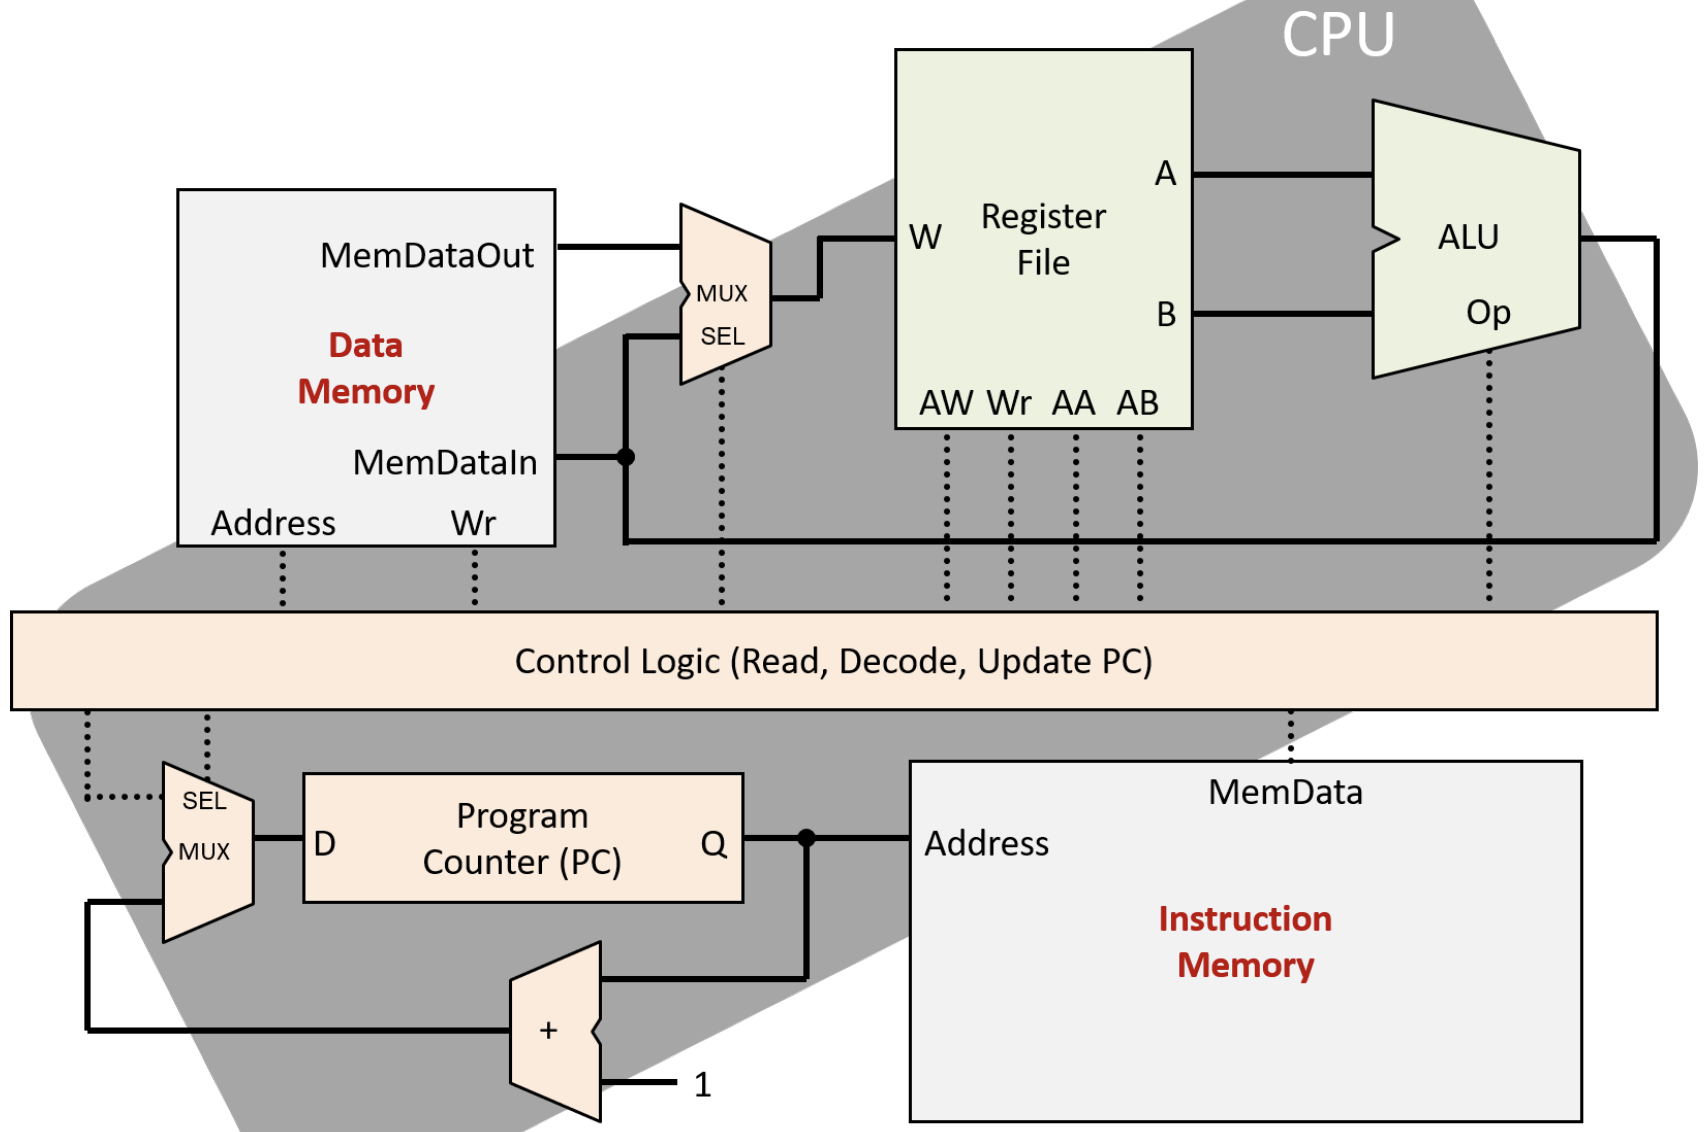
\includegraphics[width=1.2\textwidth]{chapters/chapter2a/images/processor.png}
    \end{center}
\end{minipage}

\subsection{Unified Memory}
\textit{In the image above, we see that the data memory and instruction memory are separate. However, a choice that is often made is to have a unified memory.}
\begin{center}
    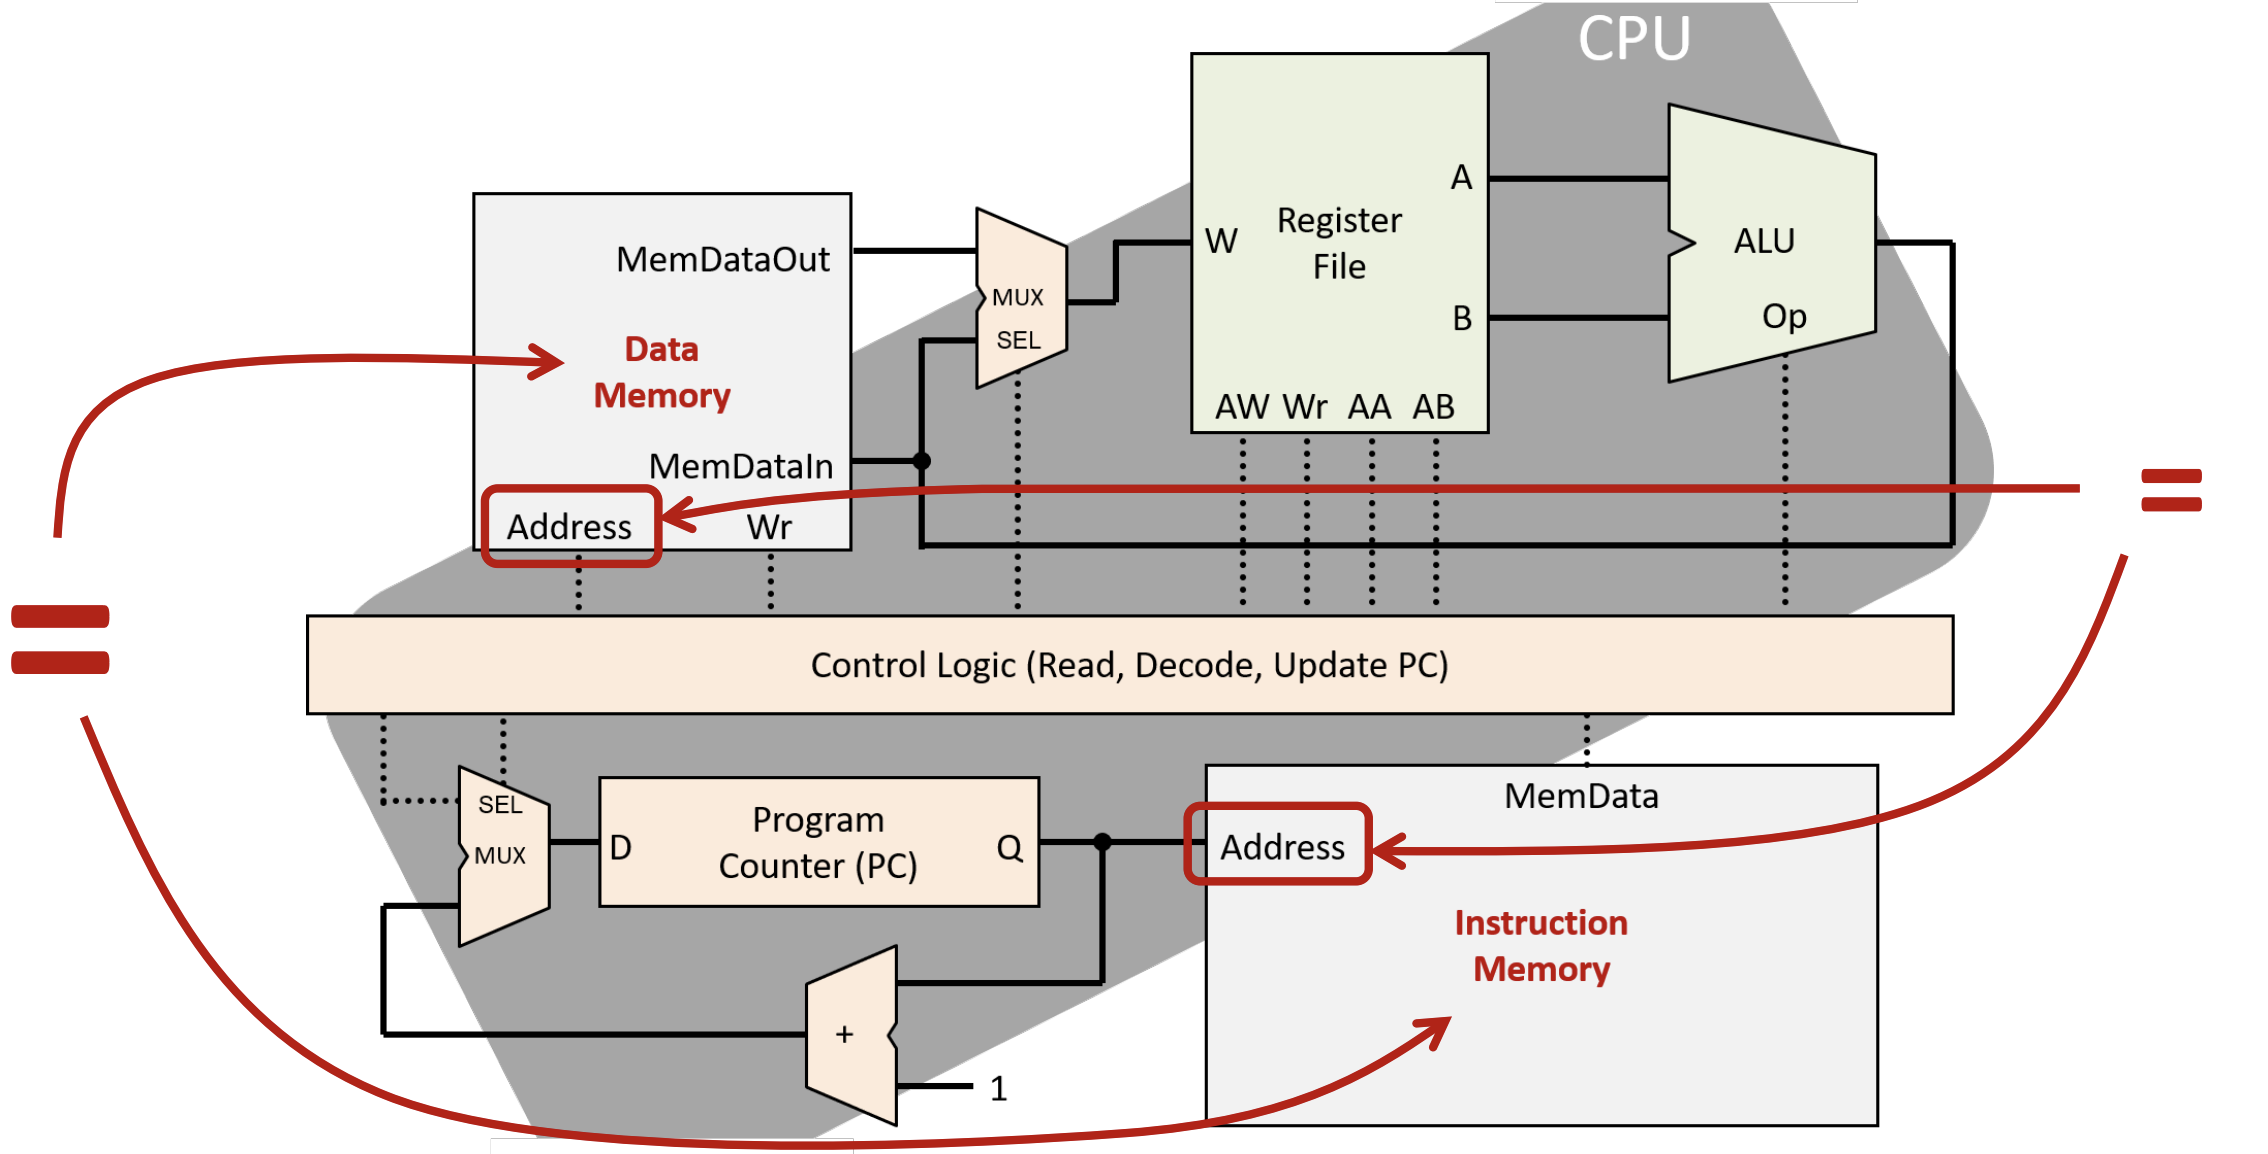
\includegraphics[width=0.75\textwidth]{chapters/chapter2a/images/unified.png}
\end{center}
\subsection{Single-Cycle Processor}
At the end, like most circuits, a processor is just another Finite State Machine. The simplified state diagram of a single-cycle processor would like this:
\begin{center}
    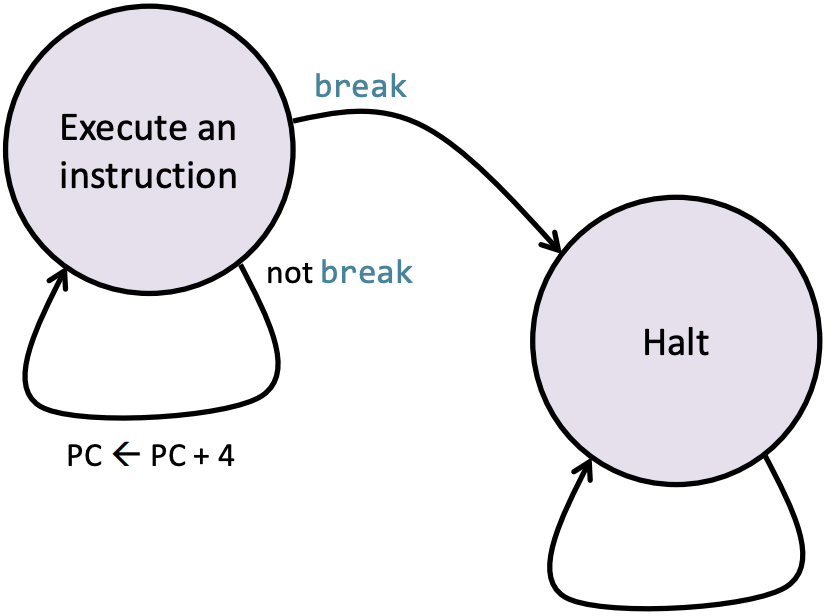
\includegraphics[width=0.35\textwidth]{chapters/chapter2a/images/fsm.png}
\end{center}
\textit{Execute an instruction, move to the next, repeat.} \\
This simplified view doesn't reflect actual CPU design. In reality, instructions take different amounts of time due to complexity and \textbf{Propagation Time}—the delay in signal travel through the processor.

\section{Propagation Time}
Remember the difference \textbf{(this is absolutely critical to understand the rest of the course)} between combinational circuits and sequential circuits. \\ \vspace*{5px} 
As the name suggests, sequential circuits are built like a \textit{sequence}(mnemotechnic), meaning the current output depends on both the current input and the previous state. \\ \vspace*{5px} 
While combinational circuits, don't have a memory, they just take an input and give out an output.  \\ \vspace*{5px}
\begin{minipage}[htp]{0.45\textwidth}
The main thing to understand here is that, for our circuits to function as intended, the \textbf{propagation time} must allow the combinational circuits to complete before the next clock cycle (otherwise, it would lead to \textit{obvious bugs}). \\ \vspace*{5px}
This implies that we need to observe the \textbf{longest combinational path} and account for it when designing our circuits.\\ \vspace*{5px}

While this is the \textit{efficient approach}, one could, in theory, design a propagation time that is longer than the longest path. However, this would result in a \textit{waste of both time and resources}.\\ \vspace*{5px}
Remember, lower propagation time means higher clock frequency, which means faster processing.
\end{minipage}
\hfill
\vline
\hfill
\begin{minipage}[htp]{0.45\textwidth}
\begin{center}
    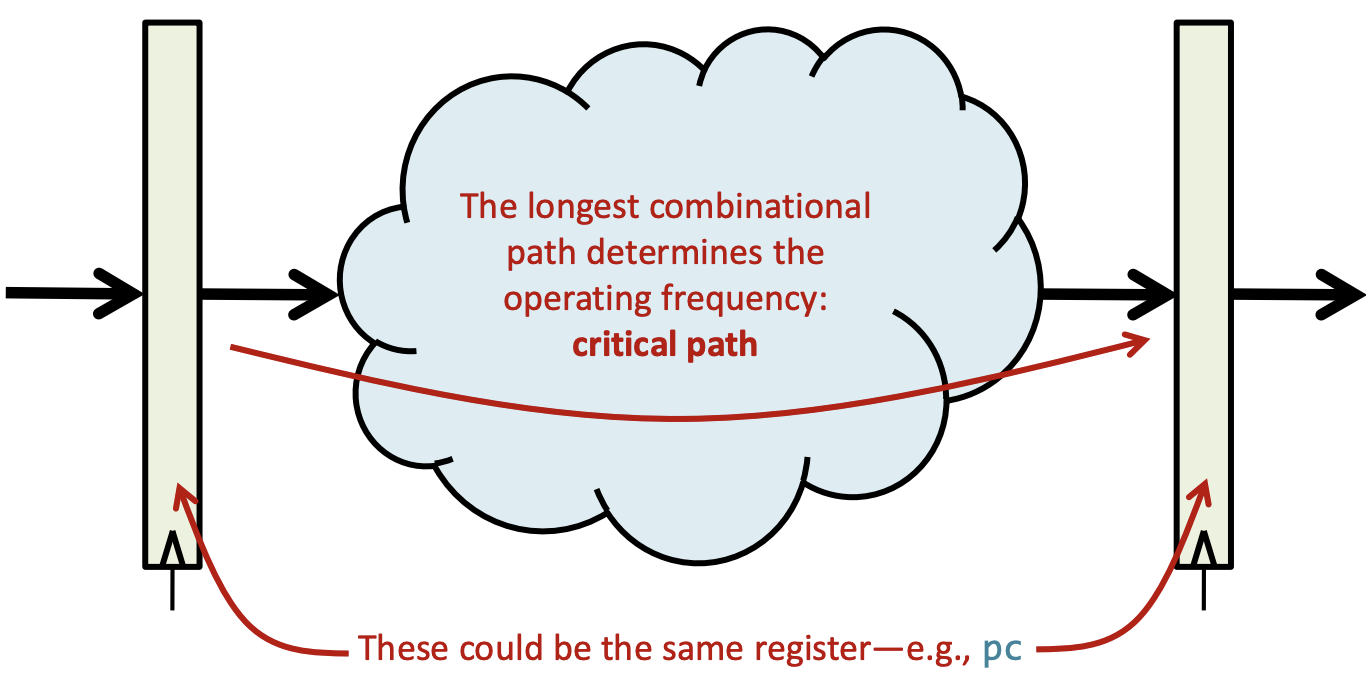
\includegraphics[width=1.2\textwidth]{chapters/chapter2a/images/prop_time.png}
\end{center}
\end{minipage}\\


\subsection{Increasing the Frequency}
To increase the frequency, we need to decrease the propagation time. This can be achieved by breaking down the combinational path into smaller parts. \\
For example, consider the `lw` instruction. This requires adding the offset to the base address (which involves addition, not completely trivial), and then reading the data from memory. This process can be broken down into two stages: first, the addition, and then the memory read. \\
\begin{center}
    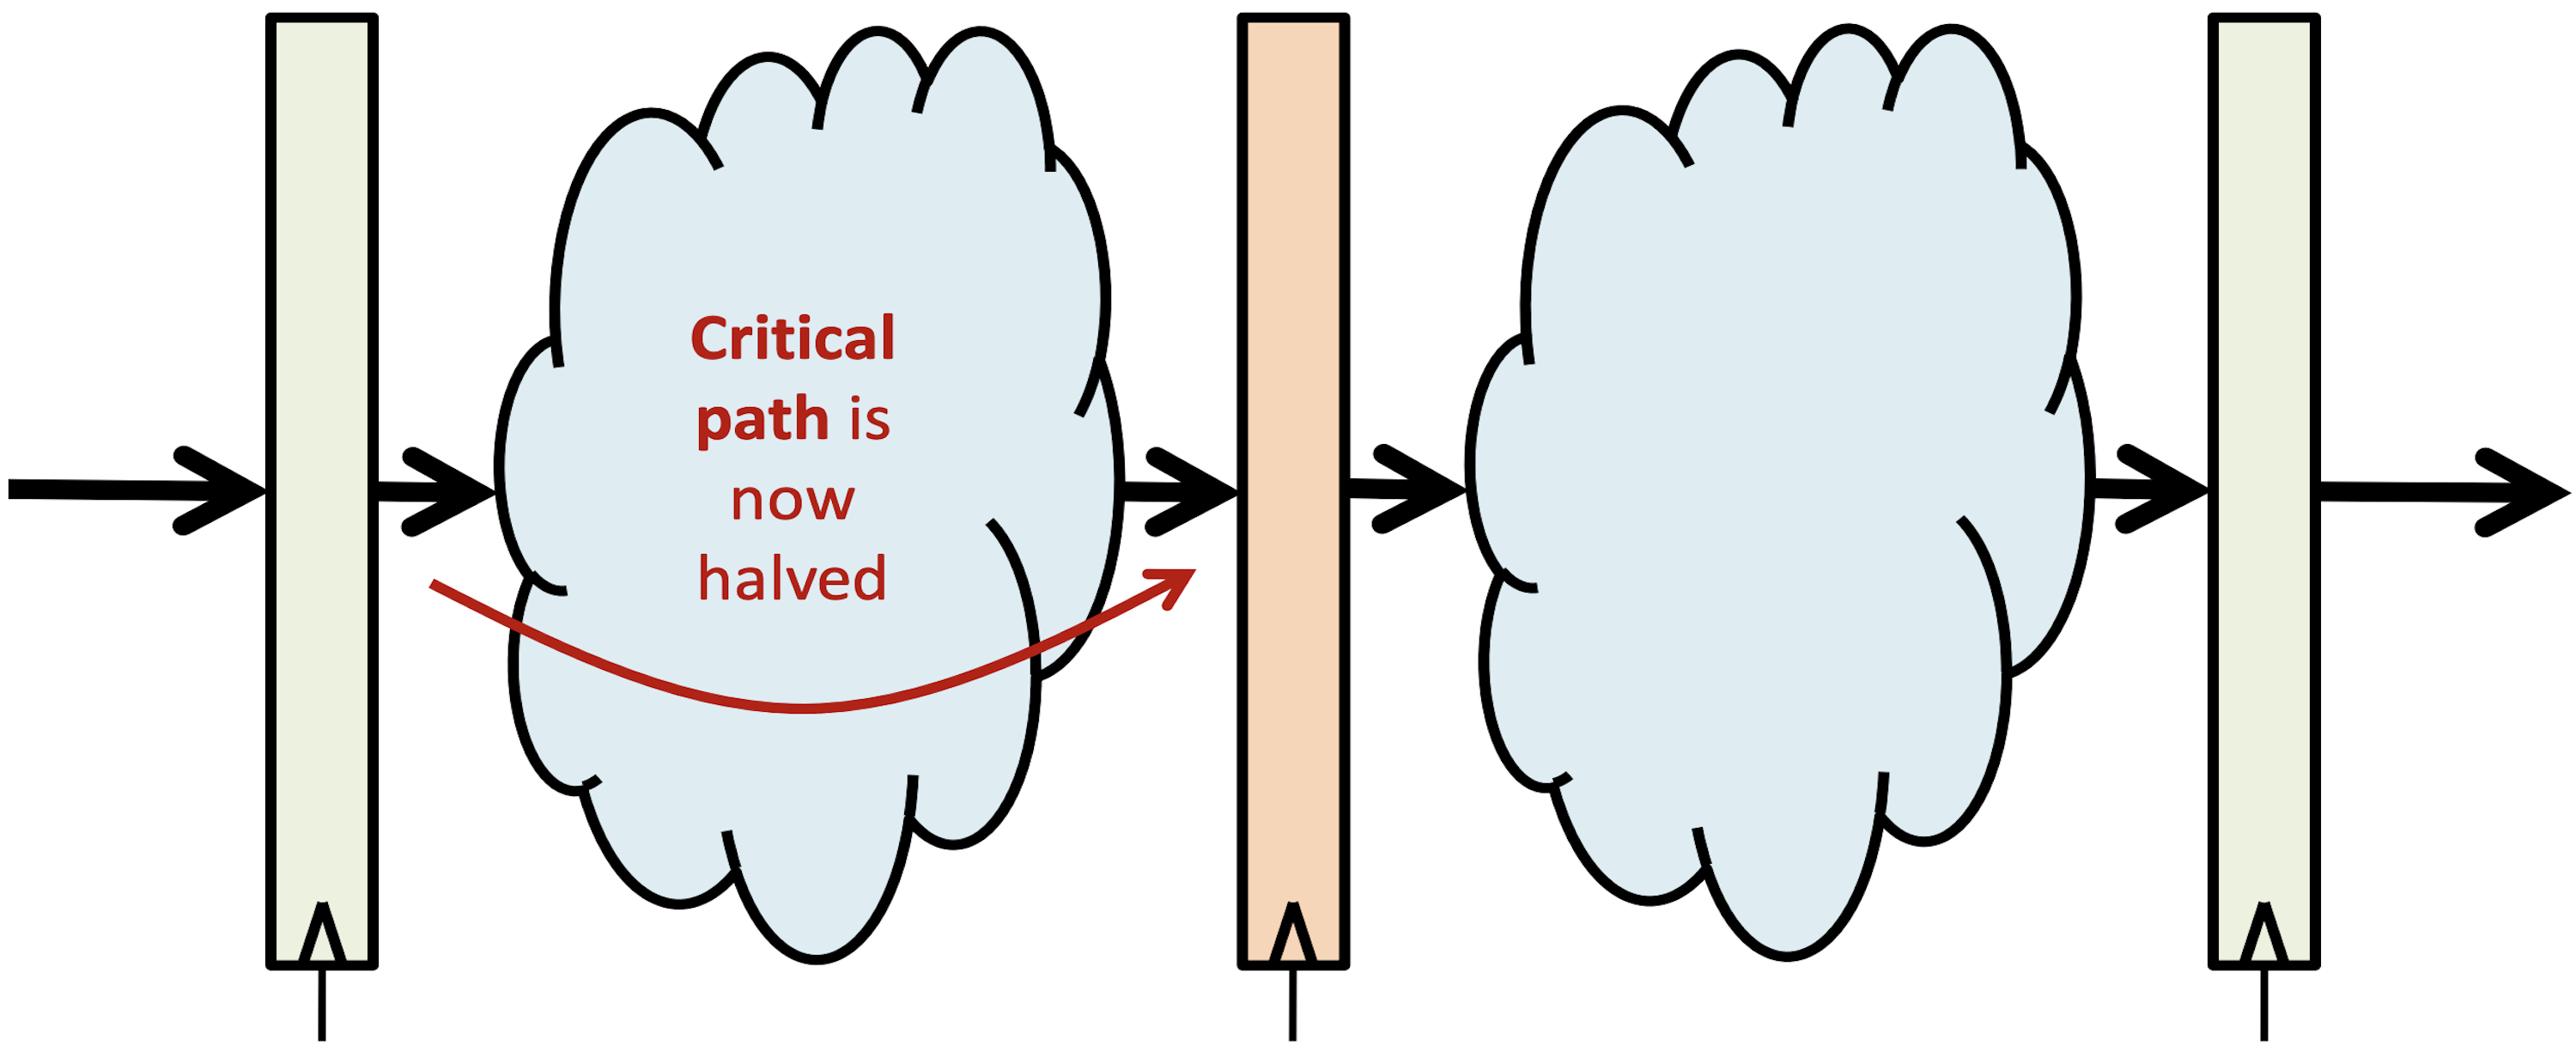
\includegraphics[width=0.45\textwidth]{chapters/chapter2a/images/incr_freq.png}
\end{center}
By doing this, we can operate at twice the \textit{""speed""}(we'll see why this is wrong in a moment). \\

\subsection{Two-Cycle Processor}
However, what we quickly realize is that this approach doesn't result in a real performance gain. While the processor runs at twice the frequency, it also takes twice as long to complete the instruction, leading to no overall improvement. \\
\textit{Historically, Intel often used this strategy to persuade uninformed consumers that their processors were getting faster.} \\
\begin{center}
    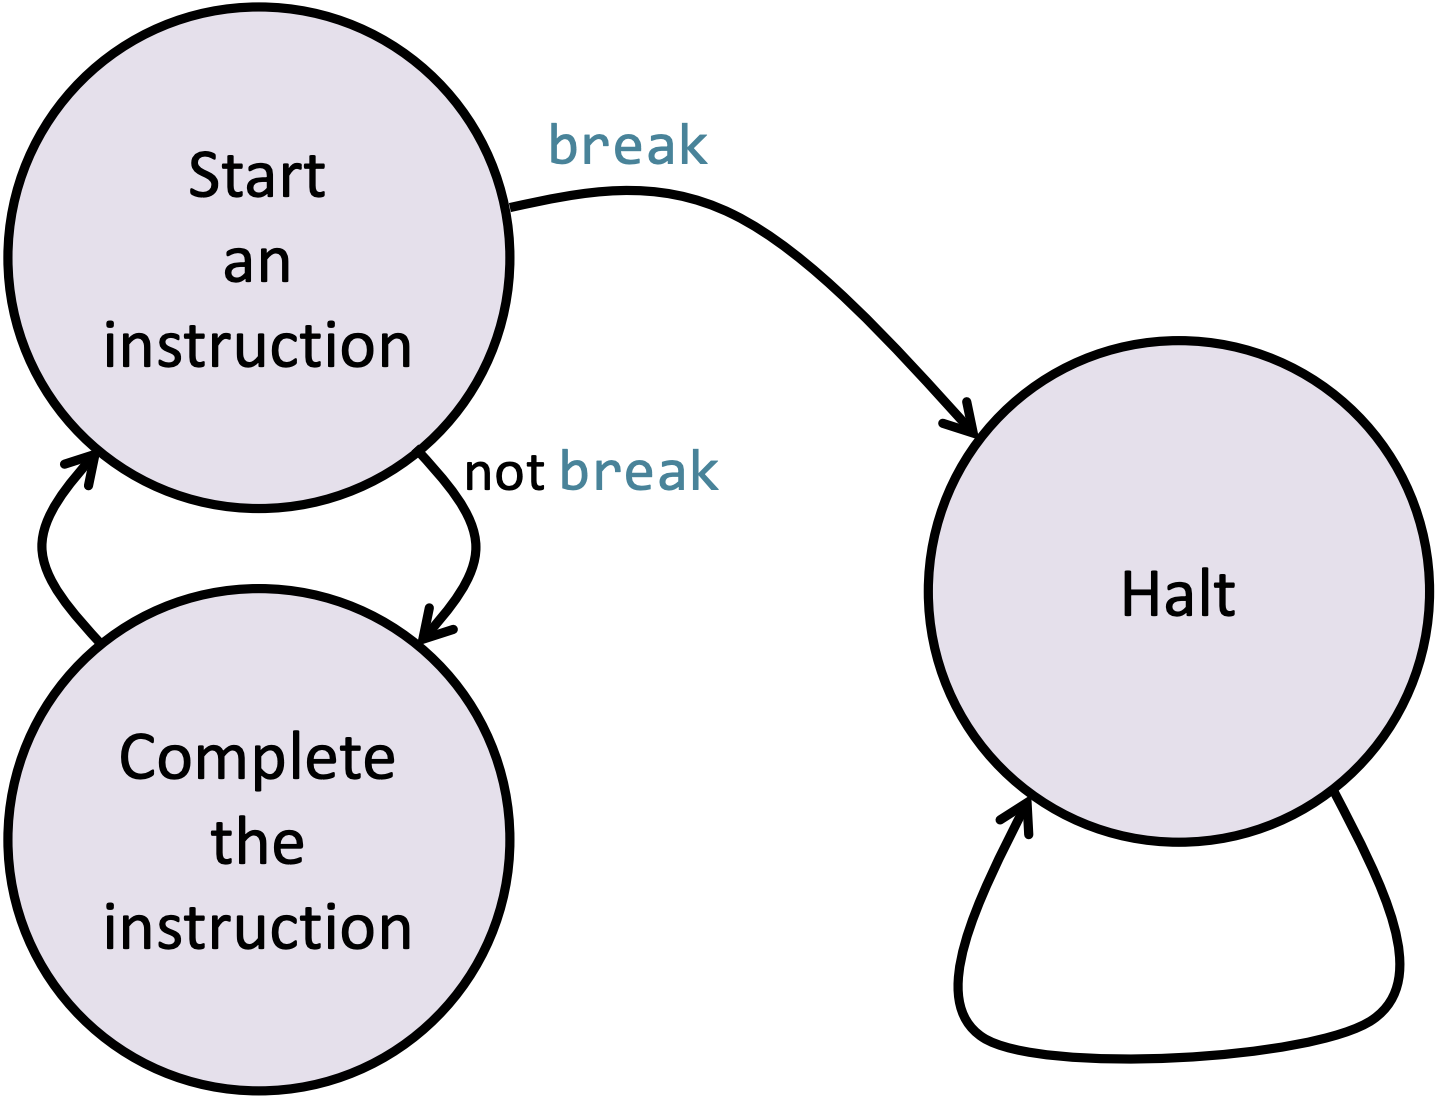
\includegraphics[width=0.45\textwidth]{chapters/chapter2a/images/two_cyc_processor.png}
\end{center}

\subsection{Not All Paths Are Born Equal}
The reason we're discussing this is that not all paths are equal. Some instructions are faster to compute than others. \\
For example, the \texttt{andi} instruction is much faster than the \texttt{lw} instruction. \\
\begin{center}
    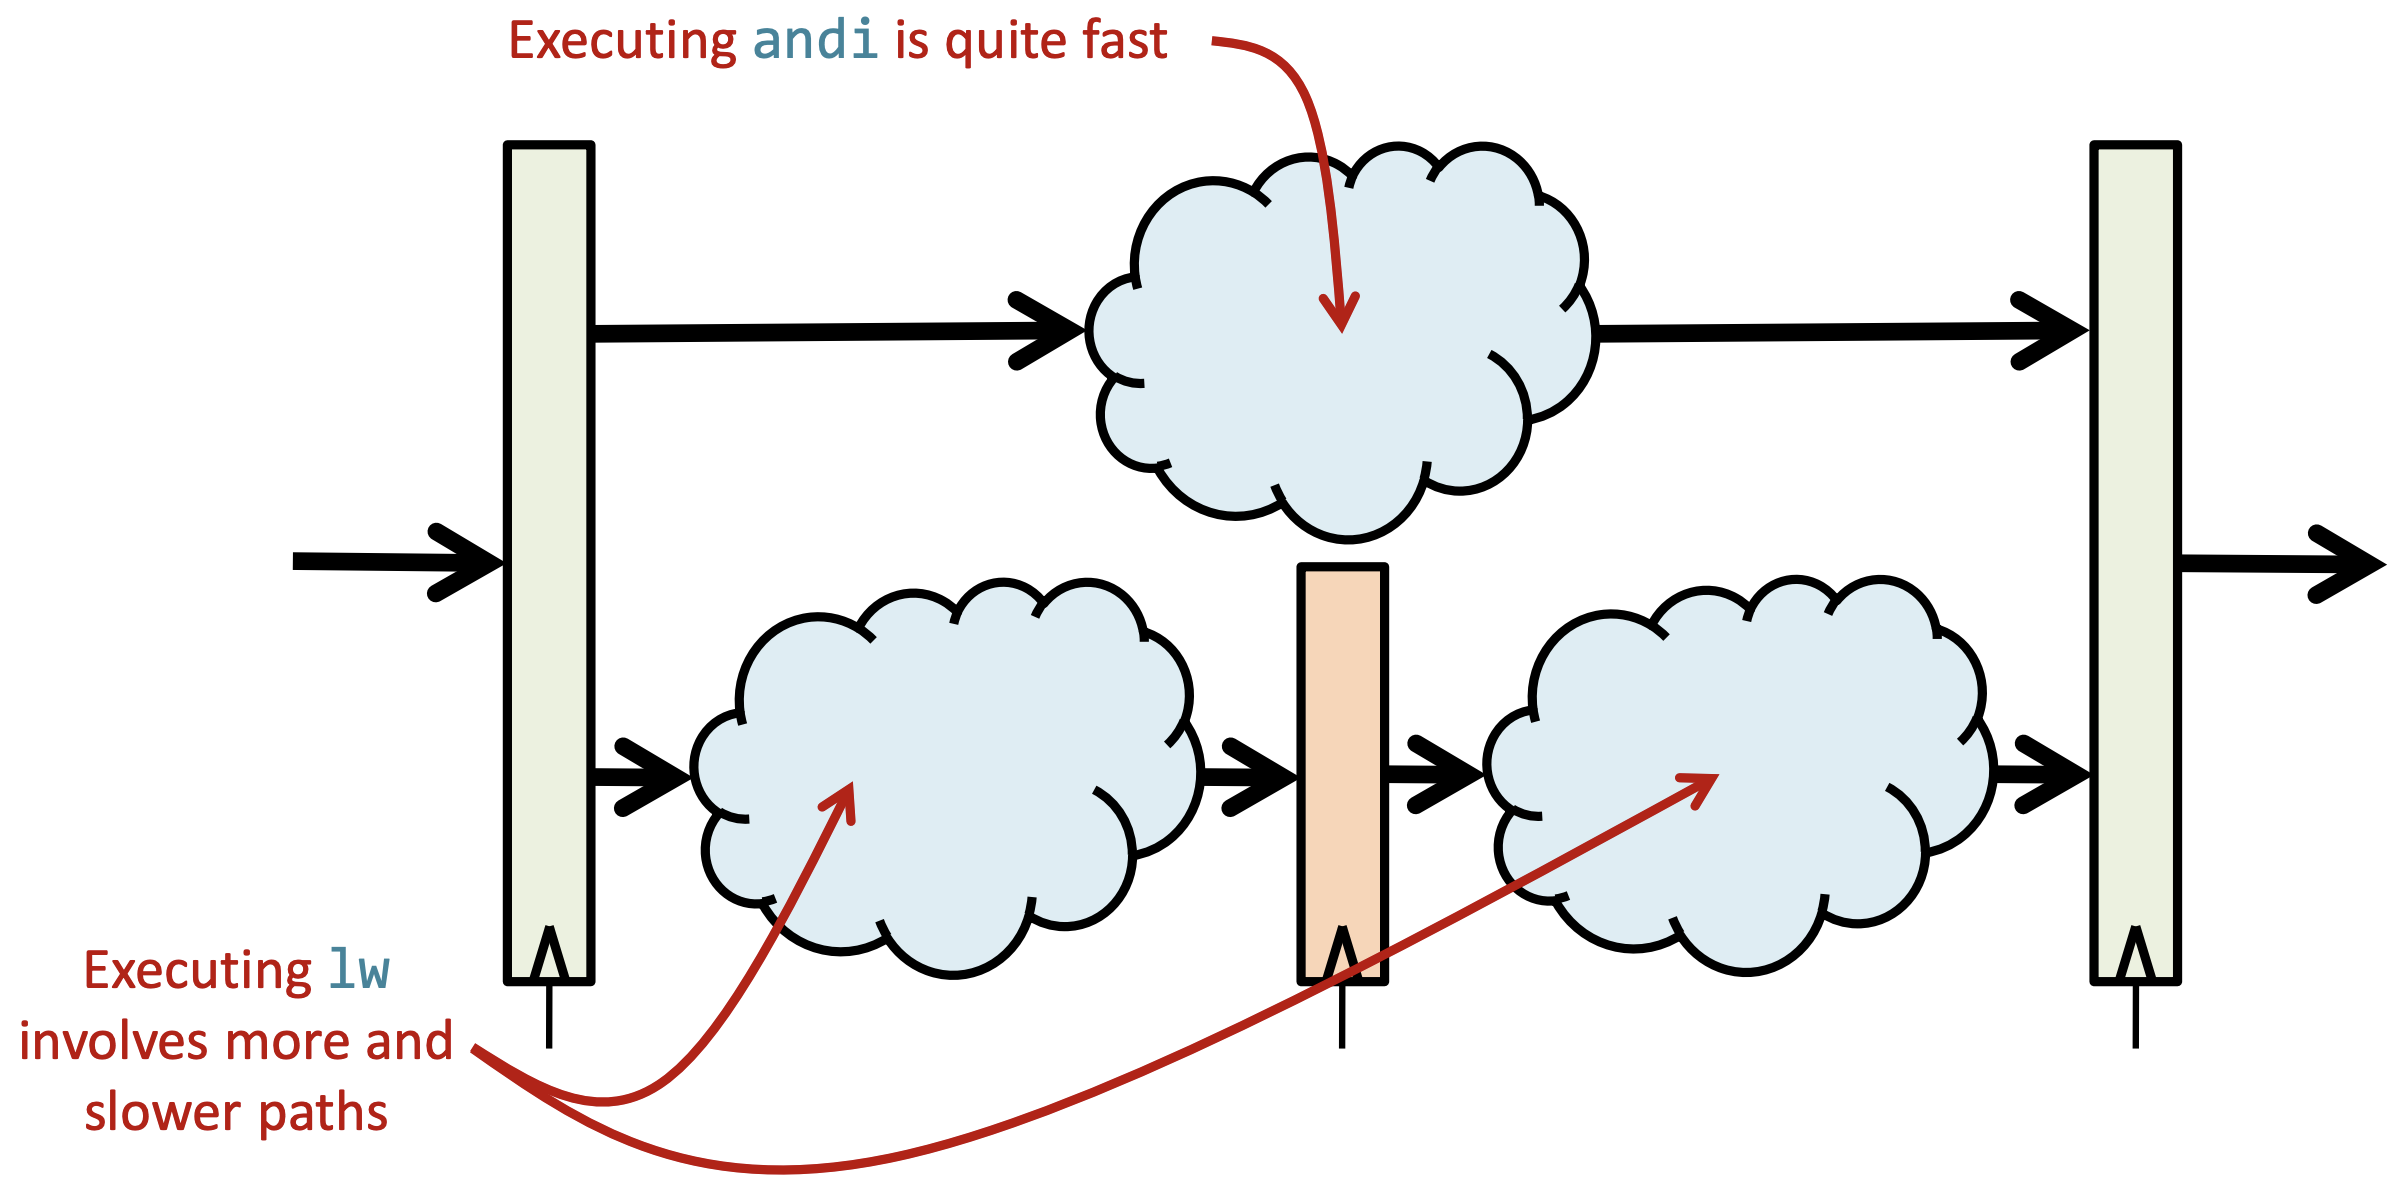
\includegraphics[width=0.65\textwidth]{chapters/chapter2a/images/paths.png}
\end{center}

\subsection{Asynchronous/Synchronous Memories}
Another reason why breaking down the combinational path could be beneficial is that certain memories are \textbf{Synchronous}, meaning they only read data from a valid memory address on the rising edge of the clock cycle. \\ 
On the other hand, \textbf{Asynchronous} memories read data as soon as a valid memory address is available, without waiting for the clock cycle.\\ \vspace*{5px}
So, for \textbf{Synchronous} memories, breaking down combinational paths into smaller segments allows us to increase the clock frequency, making memory updates faster. \\ \vspace*{5px}
\begin{minipage}[htp]{0.45\textwidth}
    \begin{center}
        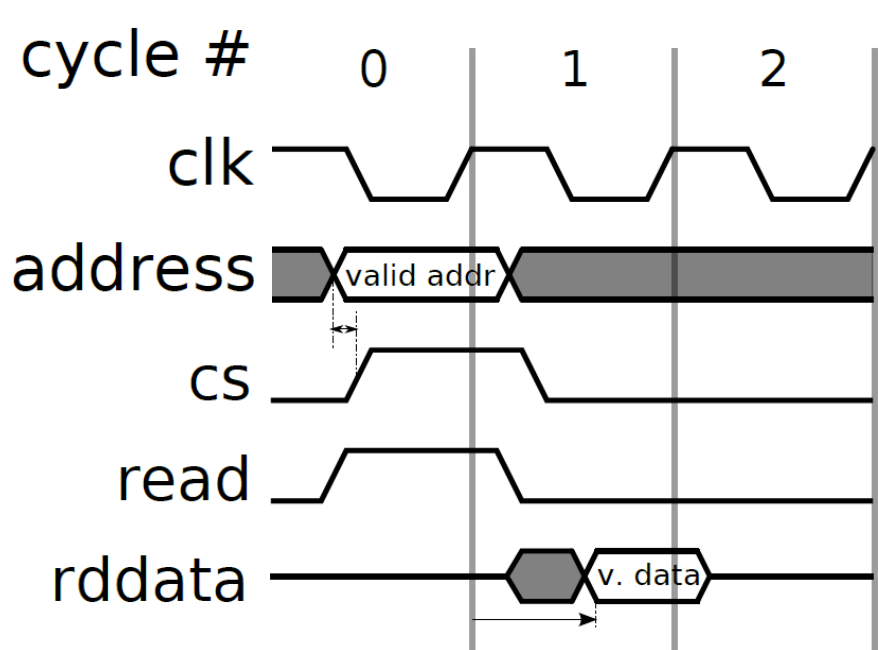
\includegraphics[width=0.65\textwidth]{chapters/chapter2a/images/seq_memory.png}
    \end{center}
\end{minipage}
\hfill
\vline
\hfill
\begin{minipage}[htp]{0.45\textwidth}
    \begin{center}
        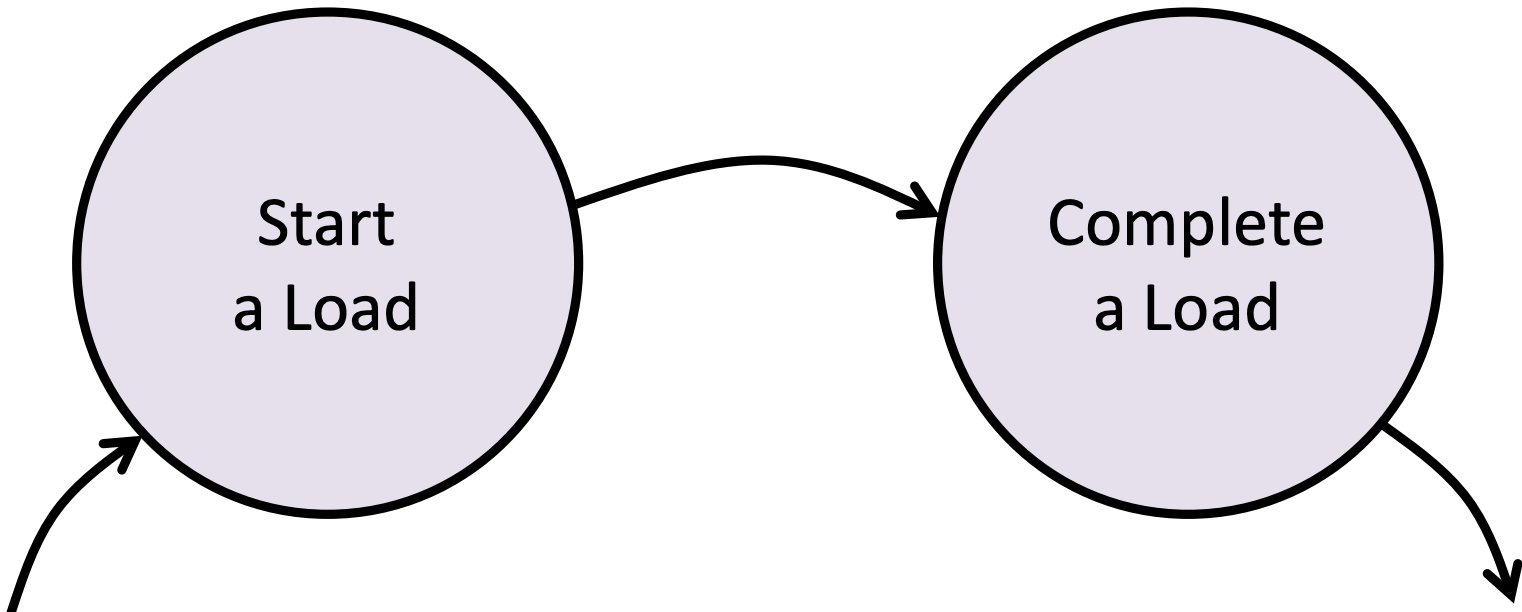
\includegraphics[width=0.85\textwidth]{chapters/chapter2a/images/seq_memory2.png}
    \end{center}
\end{minipage}

\section{Multicycle Processor}
\textit{Now let's try to construct a more convincing representation for our processor.}

The processor operates in two cycles: a faster path for simple instructions and a slower path for more complex ones. \\
\begin{minipage}[htp]{0.45\textwidth}
\vspace*{5px}
\footnotesize
\begin{justify}
        - \textbf{Fetch1/Fetch2}: 
        \begin{itemize}
        \item[] \textit{Simple}: Uses only Fetch1 for single-word instructions.
        \item[] \textit{Complex}: Uses Fetch2 to fetch additional data when needed (e.g., multi-word instructions).
        \end{itemize}
    
        - \textbf{Decode}: 
        \begin{itemize}
        \item[] \textit{Simple}: Quick decoding with fewer control signals.
        \item[] \textit{Complex}: More control signals and operands, requiring extra decoding time(and extra Optimization could be to introduce two Decoding stages for simple/complex instructions).
        \end{itemize}
    
        - \textbf{Execute}: 
        \begin{itemize}
        \item[] \textit{Simple}: Fast ALU operations like additions.
        \item[] \textit{Complex}: Involves branches or complex ALU operations.
        \end{itemize}
    
        - \textbf{Load1/Load2}: 
        \begin{itemize}
        \item[] \textit{Simple}: Skips Load stages if no memory access.
        \item[] \textit{Complex}: Memory operations use Load1 and Load2 to fetch and process data.
        \end{itemize}
\end{justify}
\end{minipage}
\hfill
\vline
\hfill
\begin{minipage}[htp]{0.45\textwidth}
    \begin{center}
        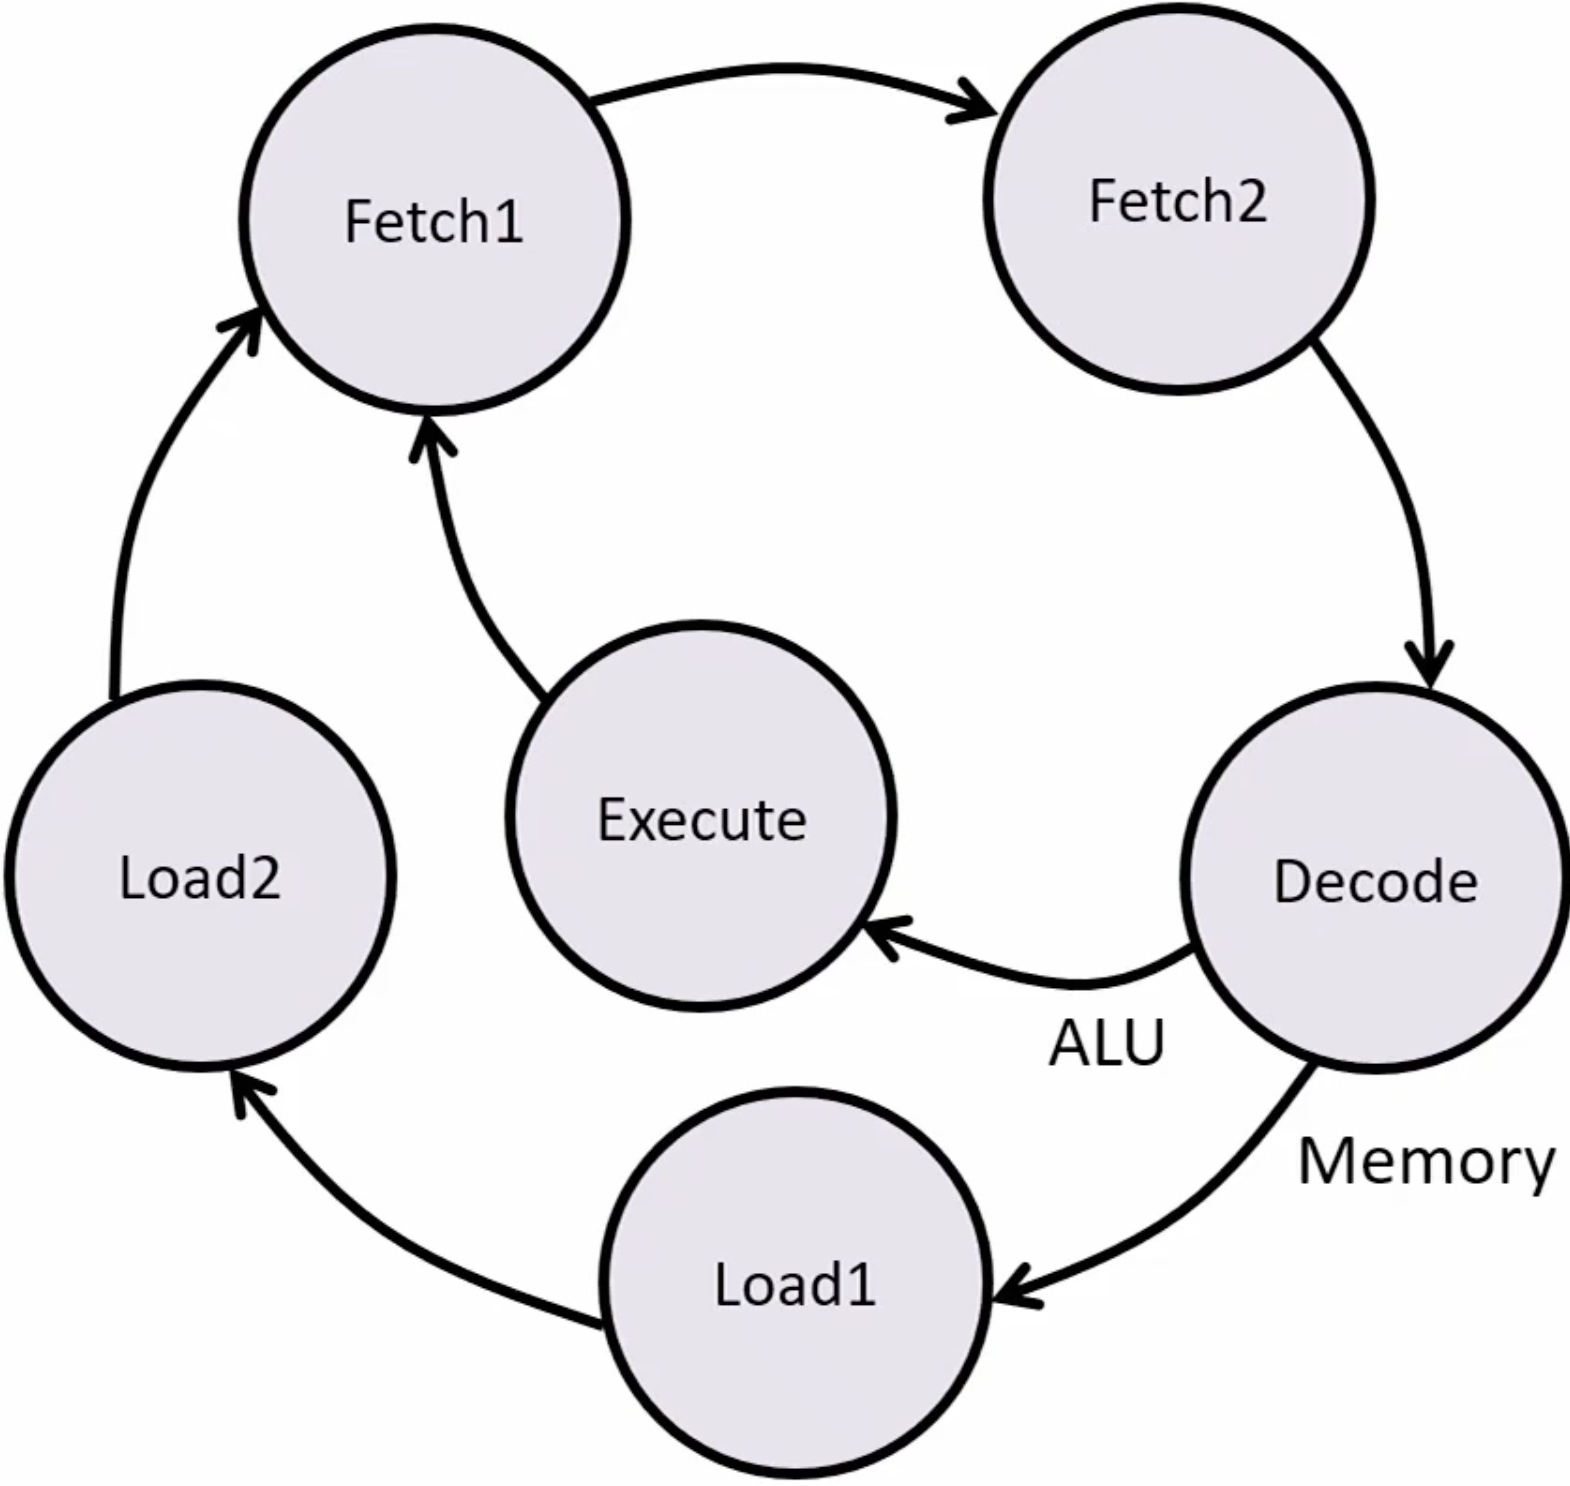
\includegraphics[width=0.70\textwidth]{chapters/chapter2a/images/multi_cyc.png}
    \end{center}
\end{minipage} \\
\vspace*{5px}
While this is an efficient design, it is not unique. The two things to keep in mind when designing a processor are: 
\begin{itemize} 
    \item[] not to have too many stages, \textit{meaning that having an excessive number of stages could increase the complexity and latency of the processor (this we will see later in the course).} 
    \item[] to have paths as balanced as possible, \textit{meaning that the duration of each stage should be similar to avoid bottlenecks that would slow down the overall process. The more balance we have the more we can profit from fast cases.} 
\end{itemize}
\newpage
\section{Mealy or Moore?}
\textit{Personal Remark (mnemotechnic)} \\
\textit{Moore - Output Only depends on state (double O like in Moore),}\\
\textit{Mealy - Output depends on state and input}\\
\begin{center}
    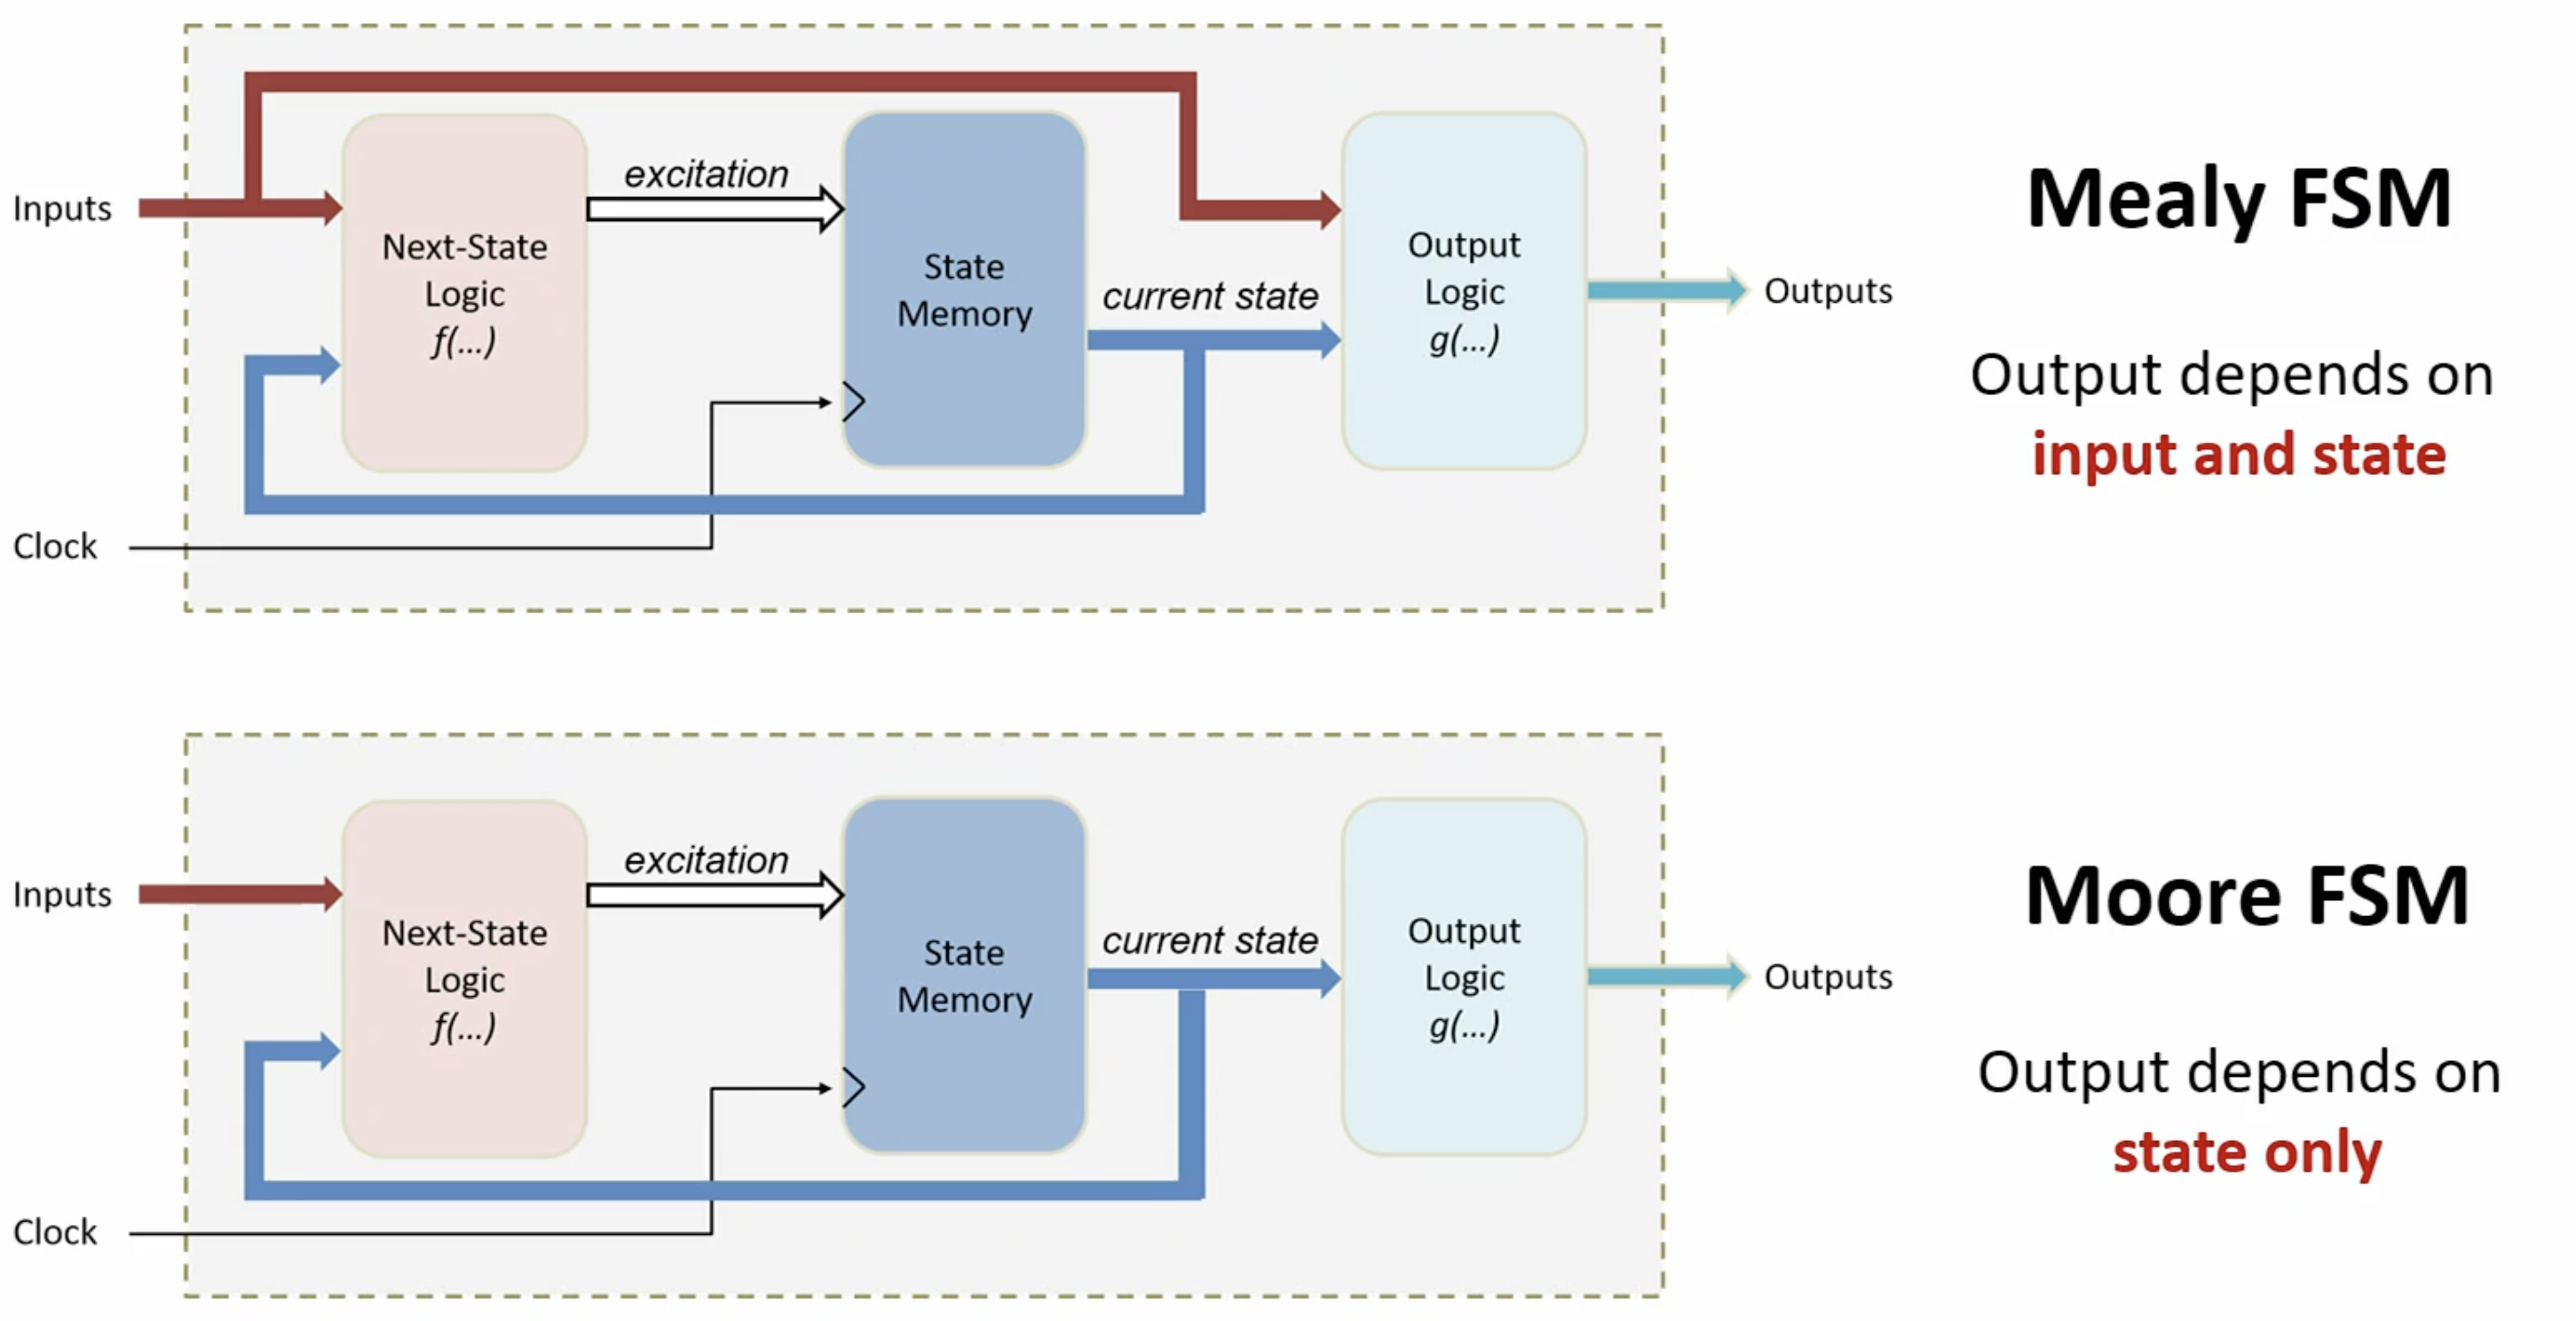
\includegraphics[width=1\textwidth]{chapters/chapter2a/images/moore_mealy.png}
\end{center}
\textit{It is generally preferable to use Moore state machines because their outputs depend only on the current state, making them simpler to design, debug, and predict, whereas Mealy machines depend on both state and input, introducing complexity and potential glitches. So unless the speicifcations requires us to do otherwise, we'll generally tend to represent our state machines as Moore machines.} \\
\section{Processor - Building the Circuit}
In this part, we will be incrementally adding the components needed to build our processor circuit.  \\
\vspace*{4px}
\begin{minipage}[htp]{0.45\textwidth}
    For now, we've added two components to our CPU:\\ \vspace*{4px}
        \textbf{Controller:} This component, although empty for now, will eventually manage the flow of data and sequence of operations within the CPU. It will control how data moves and instructions are executed. \\
        \vspace*{4px}
        \textbf{PC (Program Counter):} The PC holds the address of the next instruction to be executed from the instruction memory. It increments after each instruction fetch or is updated based on control logic. \\ \vspace*{5px}
            \textbf{Inputs} 
            \begin{itemize}
                \item \texttt{clk}: The clock input ensures the program counter updates synchronously with the system clock.
                \item \texttt{rst\_n}: An active-low reset signal that resets the program counter to a default value when low (0).
                \item \texttt{en}: The enable signal controls whether the PC updates its value (controlled by the Controller's FSM).
            \end{itemize}
            \textbf{Outputs}
            \begin{itemize}
                \item \texttt{addr}: The address output representing the next instruction to be fetched from memory.
            \end{itemize}
    \end{minipage}
\hfill
\vline
\hfill
\begin{minipage}[htp]{0.45\textwidth}
	\begin{center}
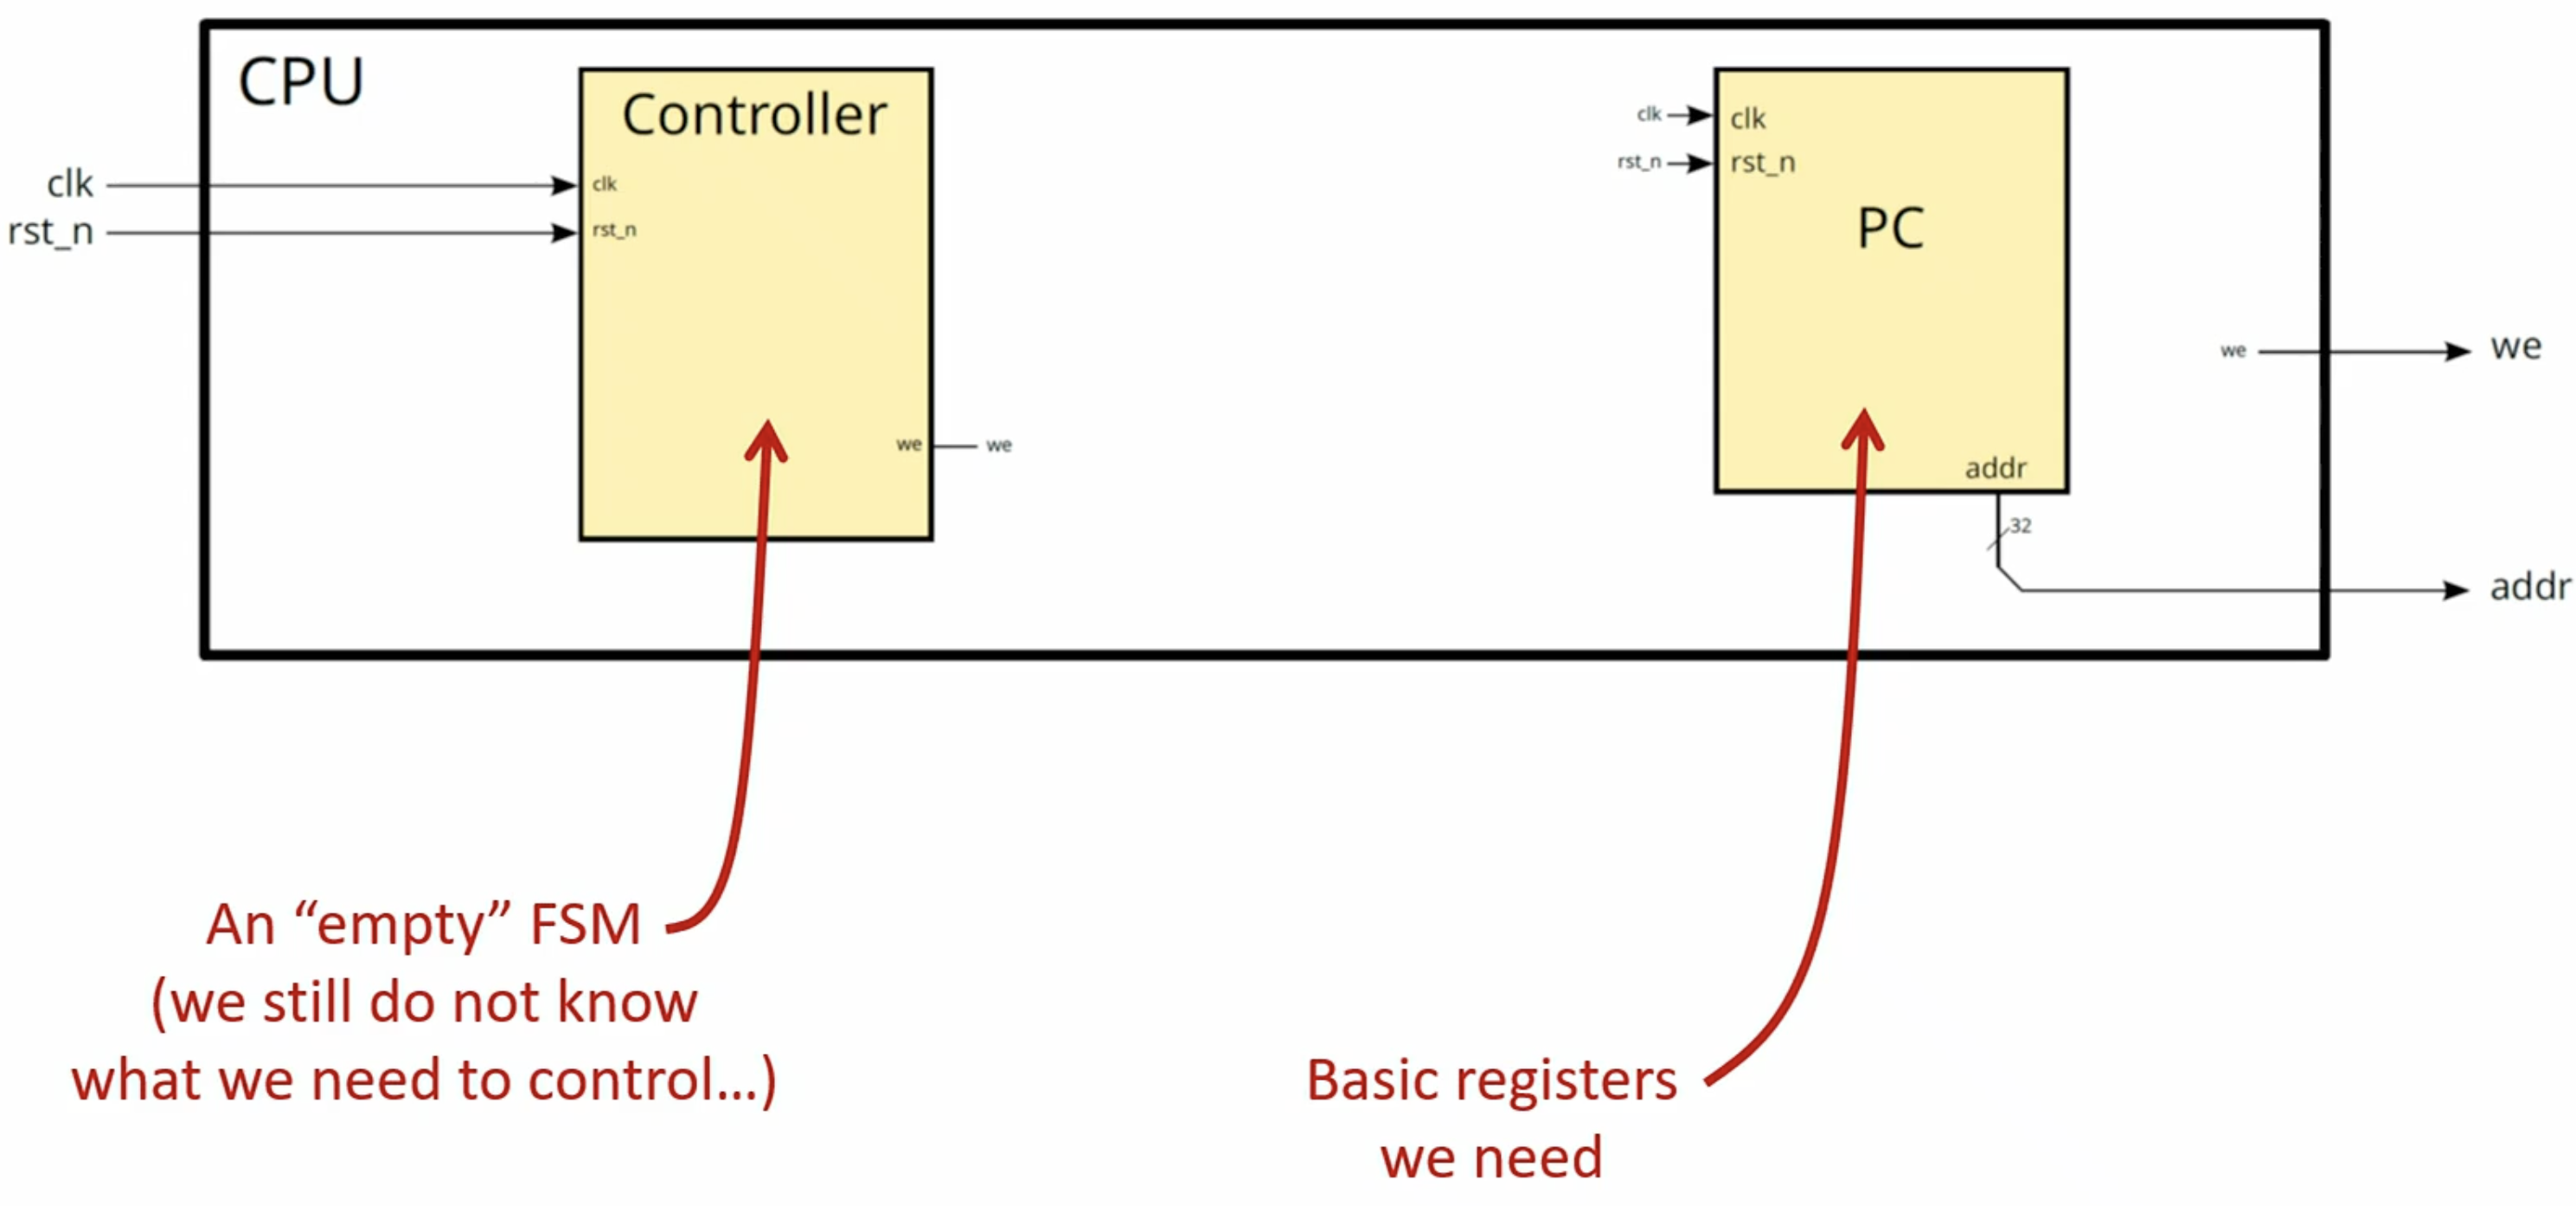
\includegraphics[width=1.2\textwidth]{chapters/chapter2a/images/p1.png}
\end{center}
\end{minipage}

\subsection{Adding the Instruction Register}
Now we're adding an Instruction Register.
\begin{center}
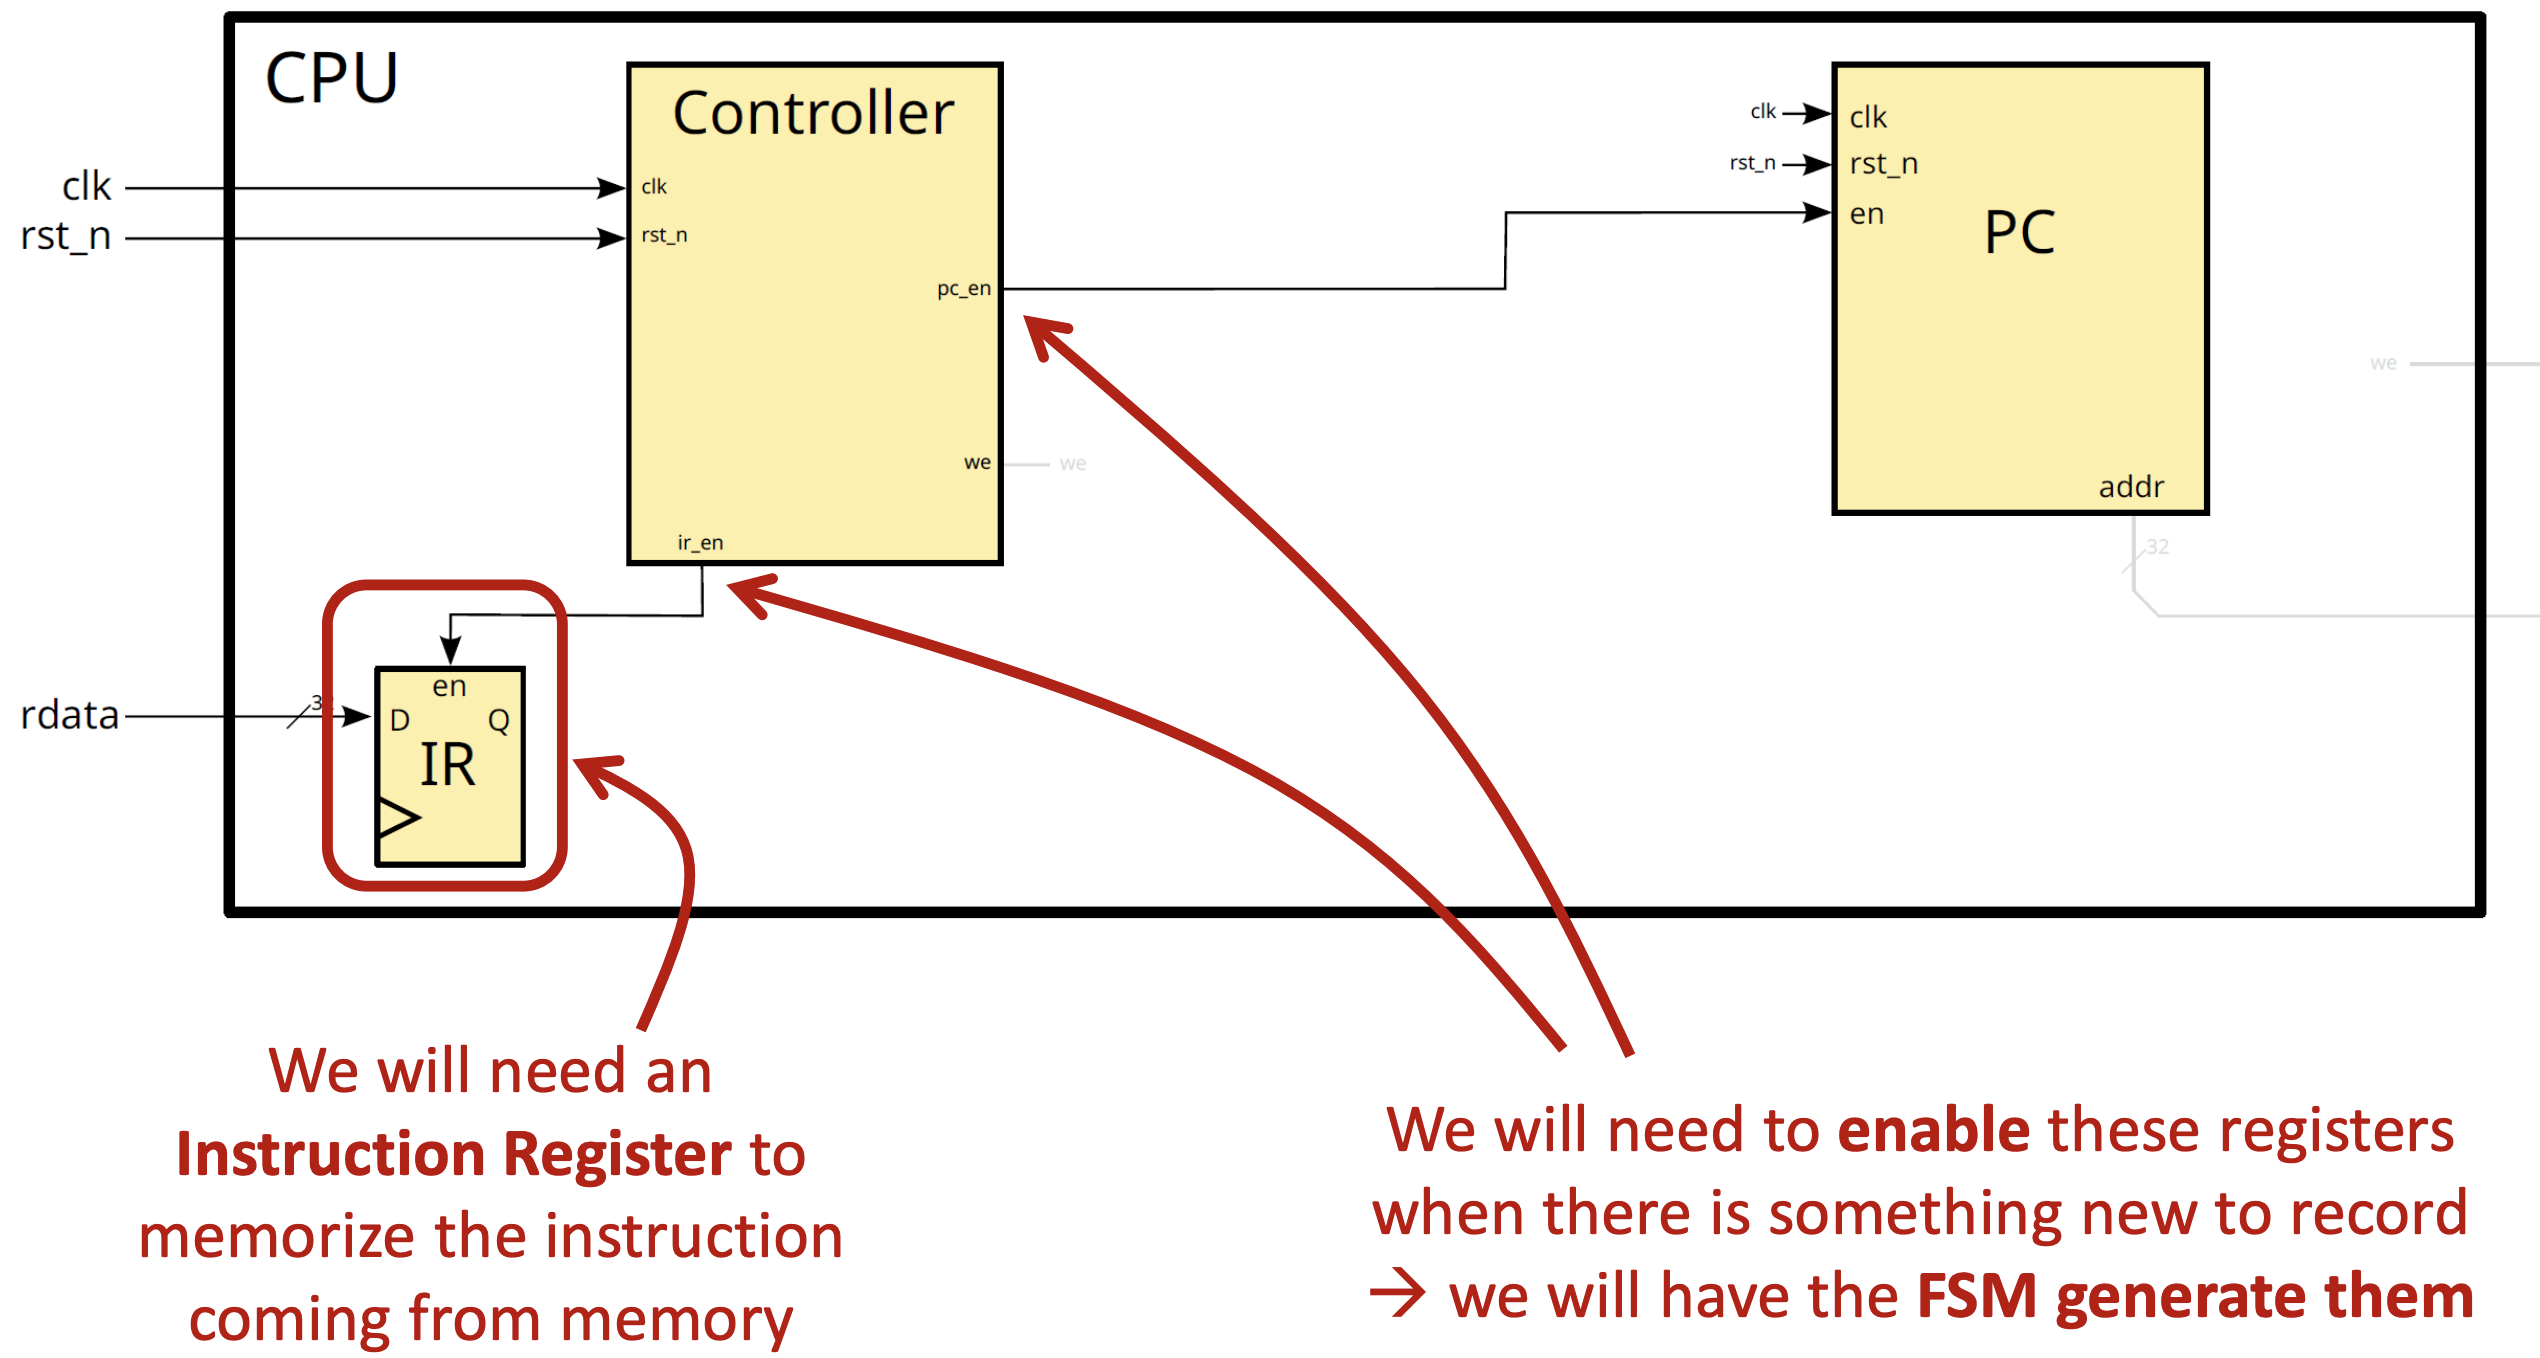
\includegraphics[width=0.75\textwidth]{chapters/chapter2a/images/p2.png}
\end{center}
In this step, we introduce the Instruction Register (IR) to our CPU: \\
\textbf{Instruction Register (IR):} The IR is responsible for storing the instruction fetched from memory. It captures the instruction ready to be decoded and executed. The Controller generates enable signals to control when the PC and IR should update their contents. \\
\noindent
\begin{minipage}[t]{0.3\textwidth}
    \footnotesize
    \textbf{PC (Program Counter)} \\ \vspace*{5px}
        \textbf{Inputs} 
        \begin{itemize}
            \item \texttt{clk}: The clock input ensures the program counter updates synchronously with the system clock.
            \item \texttt{rst\_n}: An active-low reset signal resets the program counter to a default value when low (0).
            \item \texttt{en}: The enable signal controls whether the PC updates its value. It is driven by the FSM in the Controller.
        \end{itemize}
         \textbf{Outputs}
        \begin{itemize}
            \item \texttt{addr}: The address output representing the next instruction to be fetched from memory.
        \end{itemize}
\end{minipage}
\hfill
\vline
\hfill
\begin{minipage}[t]{0.3\textwidth}
    \footnotesize
    \textbf{IR (Instruction Register)} \\ \vspace*{5px}
       \textbf{Inputs}
        \begin{itemize}
            \item \texttt{clk}: Ensures the instruction register captures the instruction at the correct clock edge.
            \item \texttt{rst\_n}: Active-low reset to reset the IR to its default state.
            \item \texttt{en}: The enable signal controls whether the IR updates its contents. It is activated when a new instruction is fetched from memory.
            \item \texttt{D}: The data input, which represents the instruction fetched from memory (\texttt{rdata}).
        \end{itemize}
        \textbf{Outputs}
        \begin{itemize}
            \item \texttt{Q}: The output of the instruction register, representing the stored instruction that will be decoded and executed.
        \end{itemize}

\end{minipage}
\hfill
\vline
\hfill
\begin{minipage}[t]{0.3\textwidth}
    \footnotesize
    \textbf{Controller} \\ \vspace*{5px}
        \textbf{Inputs}
        \begin{itemize}
            \item \texttt{clk}: The clock signal to ensure synchronization with other components.
            \item \texttt{rst\_n}: The active-low reset signal to reset the controller to its initial state.
        \end{itemize}
        \textbf{Outputs}
        \begin{itemize}
            \item \texttt{pc\_en}: The enable signal sent to the Program Counter (PC) to control when it should update its value.
            \item \texttt{ir\_en}: The enable signal sent to the Instruction Register (IR) to control when it should store a new instruction.
        \end{itemize}
\end{minipage}
\newpage
\subsection{Adding functionality}
Once an instruction is fetched from memory and stored in the Instruction Register (IR), it is crucial for the Controller to receive this instruction. The Controller needs the instruction to determine the next sequence of operations, as the next state of the system is dependent on the instruction being executed. \\
\begin{minipage}[htp]{0.45\textwidth}
    The \texttt{Q} output of the IR, which holds the stored instruction, is fed directly to the Controller. This connection allows the Controller to decode the instruction and control the subsequent operations of the CPU. \\
Specifically, the Controller will enable or disable other components, such as the Program Counter (PC), based on the instruction being processed.

\end{minipage}
\hfill
\vline
\hfill
\begin{minipage}[htp]{0.45\textwidth}
    \begin{center}
        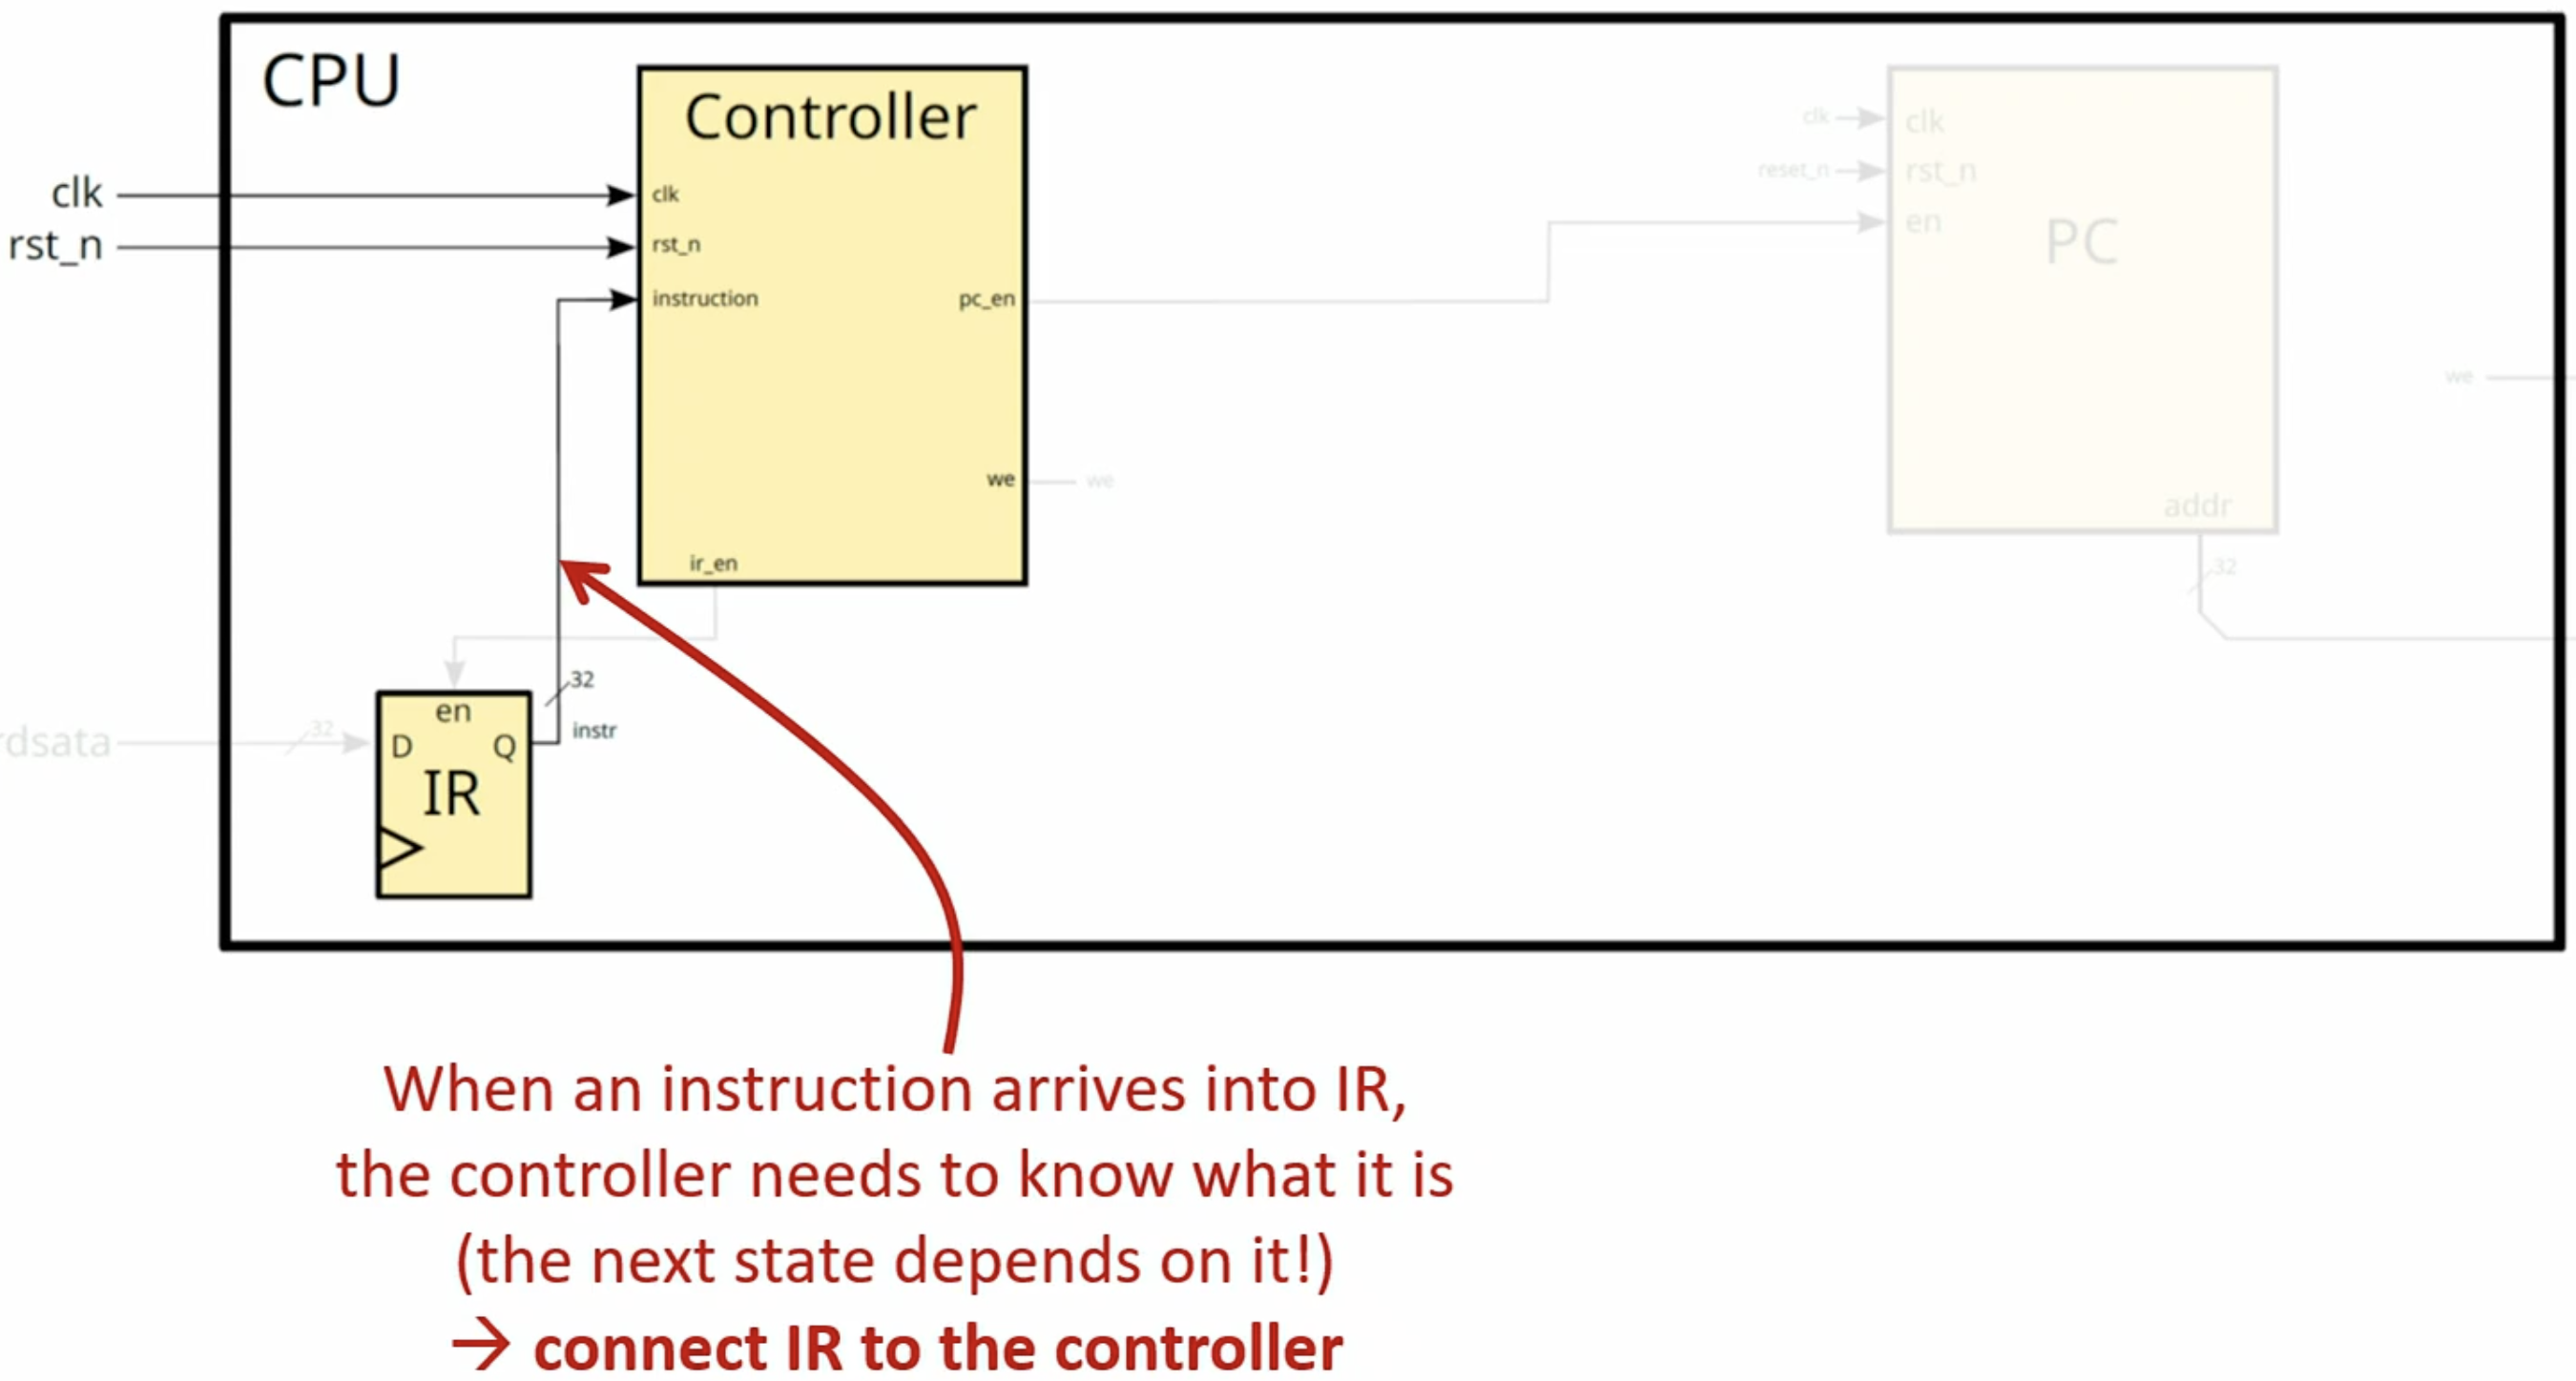
\includegraphics[width=1.2\textwidth]{chapters/chapter2a/images/p3.png}
    \end{center}
        
\end{minipage}


\subsection{I-Type Instructions Need RF and ALU}
I-Type instructions such as \texttt{addi t0, t1, 1234} require both the register file (RF) and the Arithmetic Logic Unit (ALU) for execution. The operation consists of an addition between a register value and an immediate value, and the result is stored back into a register.
\begin{center}
    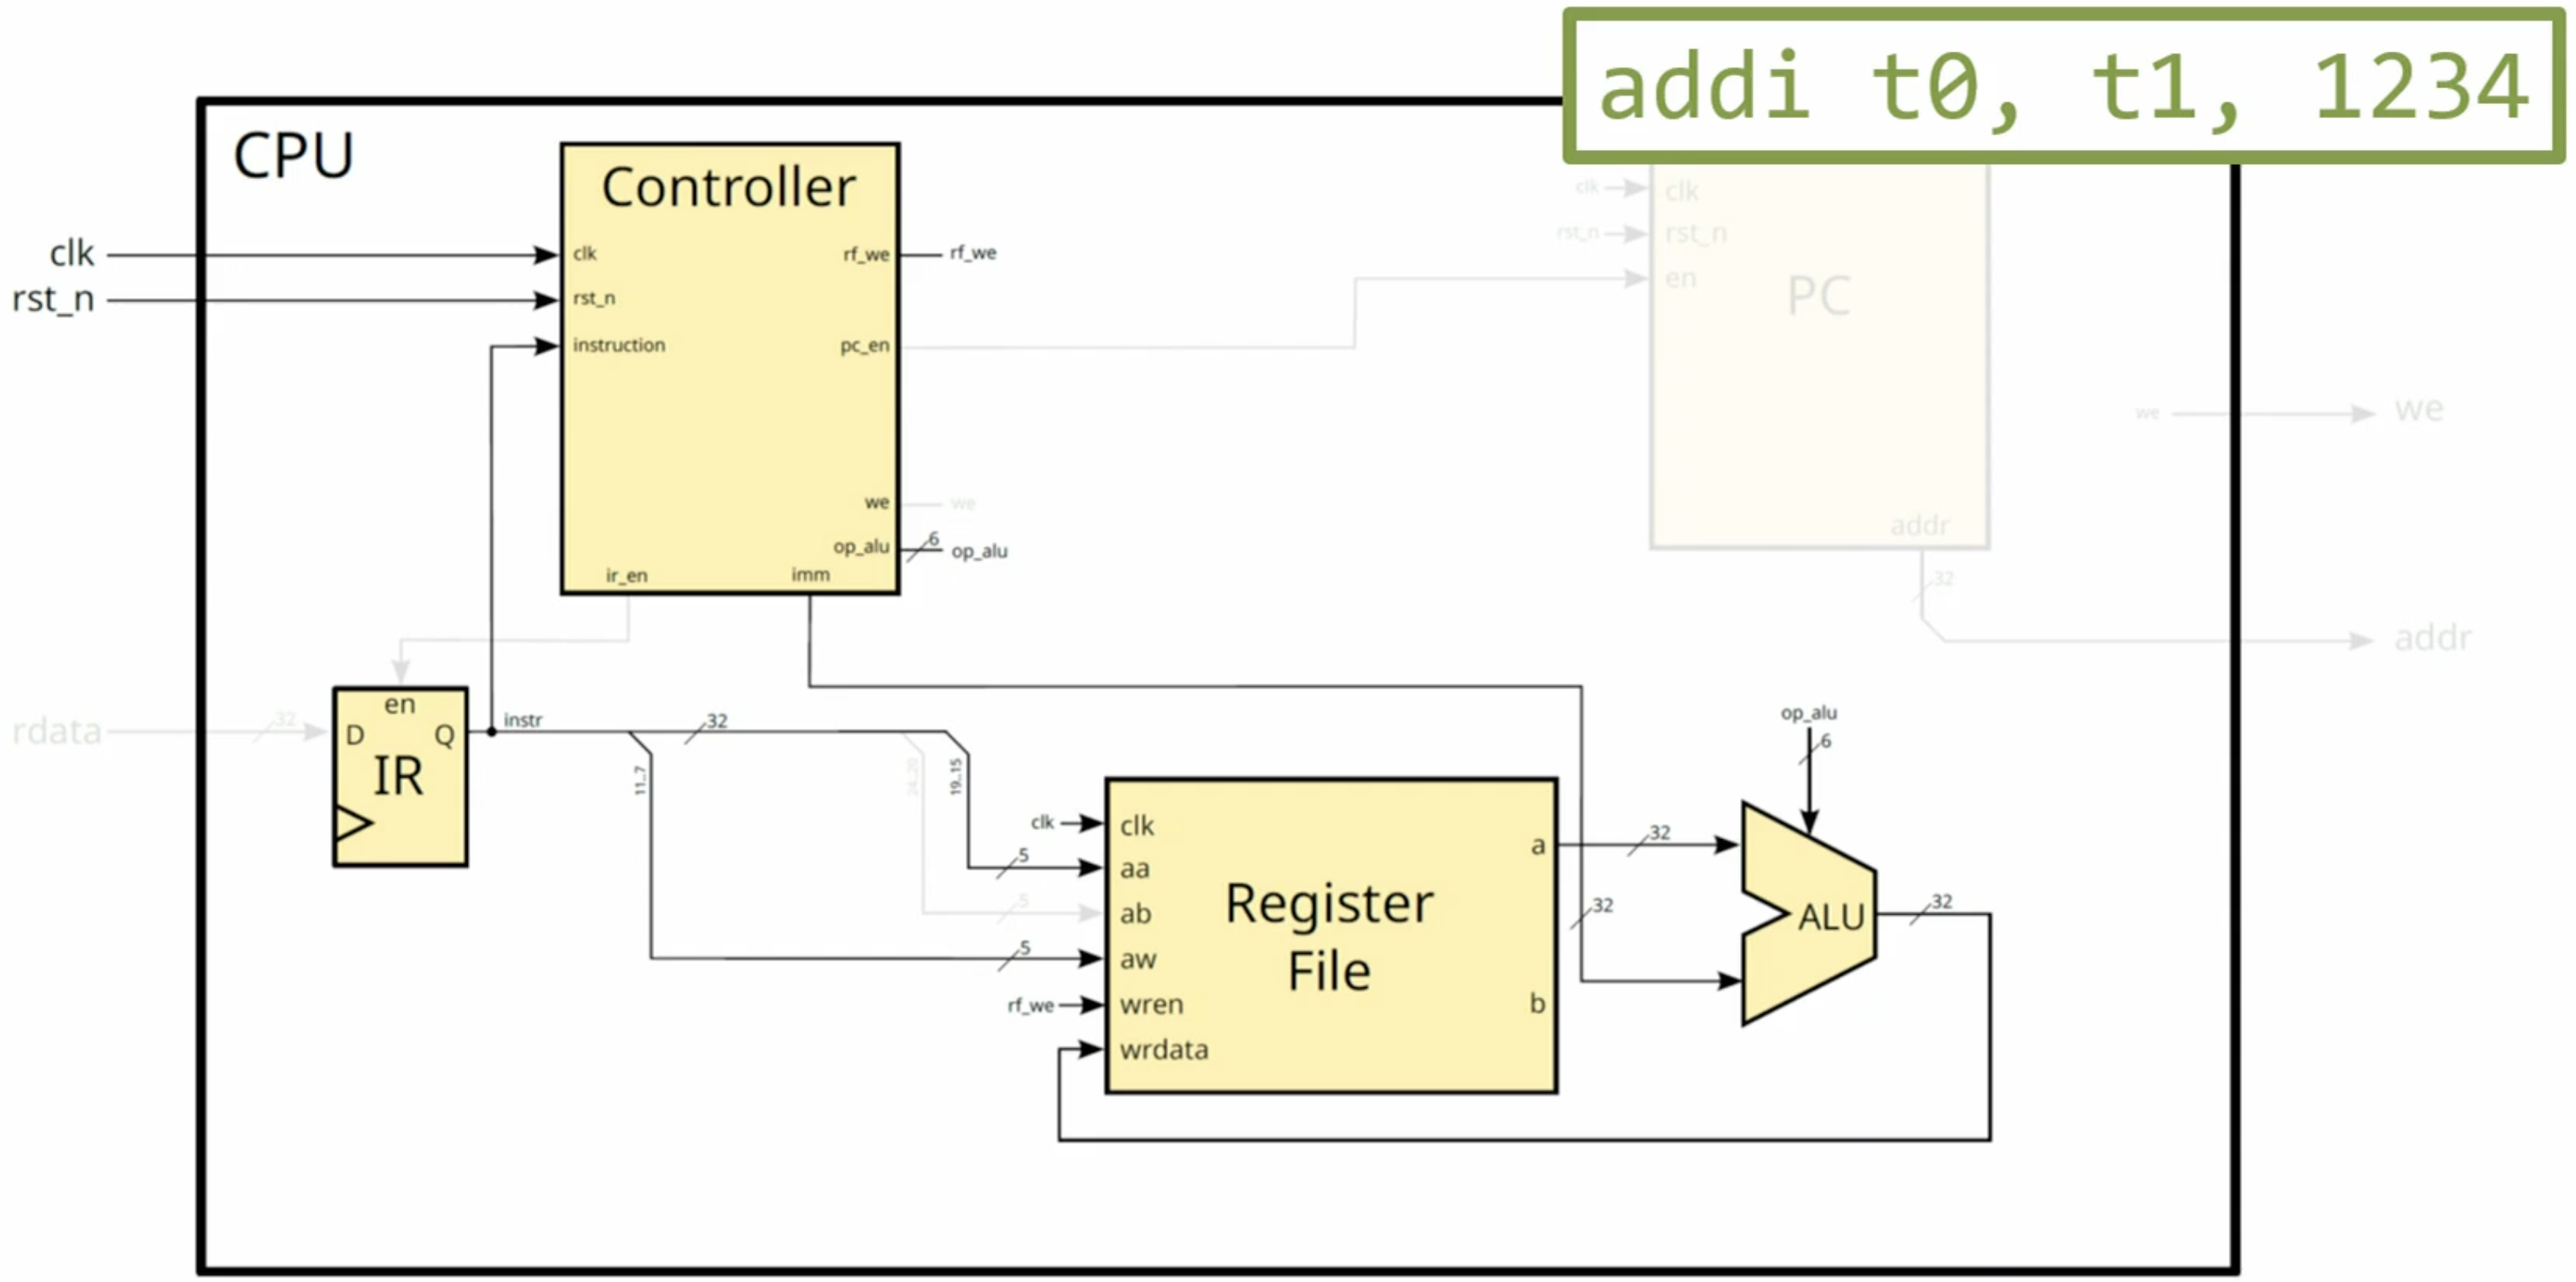
\includegraphics[width=0.5\textwidth]{chapters/chapter2a/images/p4.png}
\end{center}
\noindent
\begin{minipage}[t]{0.45\textwidth}
    \footnotesize
    \textbf{ALU (Arithmetic Logic Unit)} \\ \vspace*{5px}
        \textbf{Inputs} 
        \begin{itemize}
            \item \texttt{a}: First operand input from the register file (e.g., \texttt{t1}).
            \item \texttt{b}: Second operand input, typically the immediate value for I-type instructions (e.g., \texttt{1234}).
            \item \texttt{op\_alu}: Control signal from the controller specifying the operation to perform (e.g., addition for the \texttt{addi} instruction).
        \end{itemize}
         \textbf{Outputs}
        \begin{itemize}
            \item \texttt{alu\_out}: The result of the operation performed by the ALU (e.g., the sum of \texttt{t1} and the immediate value).
        \end{itemize}
\end{minipage}
\hfill
\vline
\hfill
\begin{minipage}[t]{0.45\textwidth}
    \footnotesize
    \textbf{Register File} \\ \vspace*{5px}
       \textbf{Inputs}
        \begin{itemize}
            \item \texttt{clk}: The clock input that ensures register updates are synchronous with the system clock.
            \item \texttt{aa}: The address of the first register (e.g., \texttt{t1}) from which data will be read.
            \item \texttt{ab}: The address of the second register (for other instruction types).
            \item \texttt{aw}: The address of the destination register (e.g., \texttt{t0}) to which the result will be written.
            \item \texttt{wren}: Write enable signal that allows data to be written into the destination register.
            \item \texttt{wrdata}: The data to be written into the destination register (e.g., the result from the ALU).
        \end{itemize}
        \textbf{Outputs}
        \begin{itemize}
            \item \texttt{a}: The data from the first register (e.g., the value stored in \texttt{t1}).
            \item \texttt{b}: The data from the second register (for other instruction types).
        \end{itemize}

\end{minipage}


\subsection{R-Type Instructions and Second Operand Selection}

R-Type instructions, such as \texttt{add t0, t1, t2}, require two register operands and involve several components for execution. The instruction specifies two source registers (\texttt{t1} and \texttt{t2}) and a destination register (\texttt{t0}), with the second operand selected from the register file rather than using an immediate value. The multiplexer plays a key role in selecting the correct second operand based on the instruction type. \\
\begin{center}
    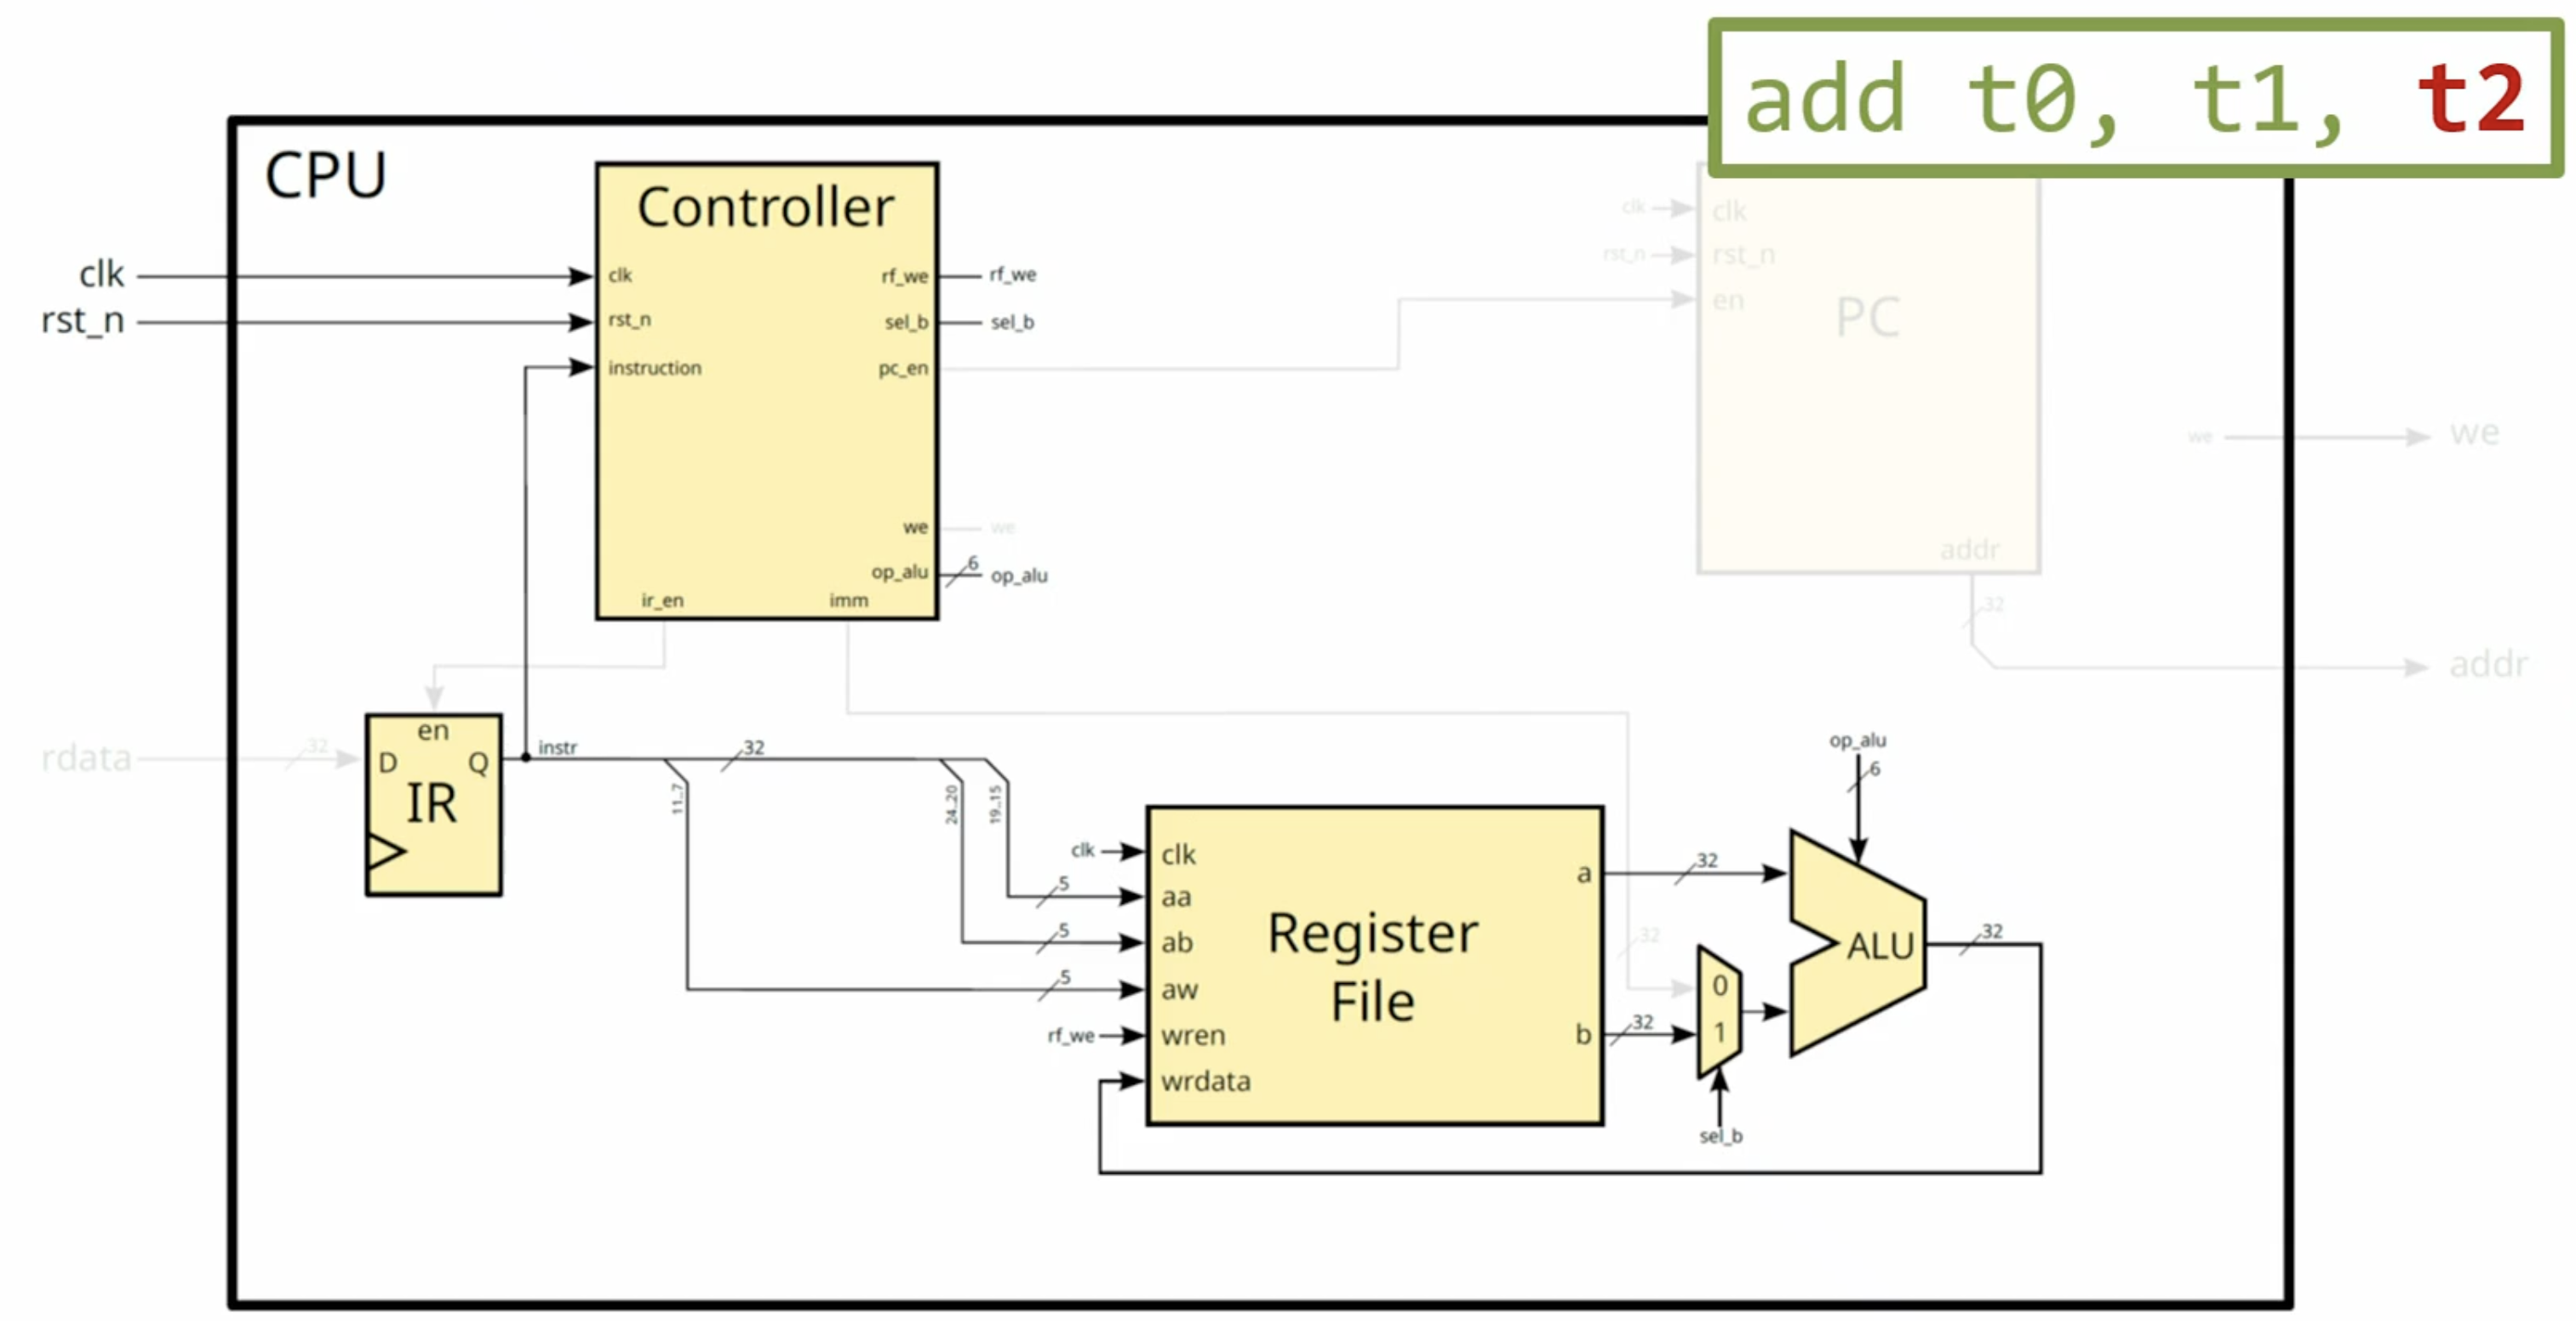
\includegraphics[width=0.75\textwidth]{chapters/chapter2a/images/p5.png}
\end{center}
\noindent

\begin{minipage}[t]{0.3\textwidth}
    \footnotesize
    \textbf{Register File} \\ \vspace*{5px}
    \textbf{Inputs}
    \begin{itemize}
        \item \texttt{clk}: The clock input that ensures register updates are synchronous with the system clock.
        \item \texttt{aa}: The address of the first register (e.g., \texttt{t1}) from which data will be read.
        \item \texttt{ab}: The address of the second register (e.g., \texttt{t2}) from which data will be read.
        \item \texttt{aw}: The address of the destination register (e.g., \texttt{t0}) where the result will be written.
        \item \texttt{wren}: Write enable signal that allows data to be written into the destination register.
        \item \texttt{wrdata}: Data to be written into the destination register (e.g., the result from the ALU).
    \end{itemize}
    \textbf{Outputs}
    \begin{itemize}
        \item \texttt{a}: The data from the first register (e.g., the value stored in \texttt{t1}).
        \item \texttt{b}: The data from the second register (e.g., the value stored in \texttt{t2}).
    \end{itemize}
\end{minipage}
\hfill
\vline
\hfill
\begin{minipage}[t]{0.3\textwidth}
    \footnotesize
    \textbf{Multiplexer (sel\_b)} \\ \vspace*{5px}
    \textbf{Inputs}
    \begin{itemize}
        \item \texttt{b}: The second operand, which can either be the register value (\texttt{t2}) or an immediate value, depending on the instruction type.
        \item \texttt{sel\_b}: The select signal from the controller, determining whether the second operand is a register value (\texttt{t2}) or an immediate value.
    \end{itemize}
    \textbf{Outputs}
    \begin{itemize}
        \item \texttt{selected\_b}: The selected operand output, which forwards either the register value (\texttt{t2}) or the immediate value to the ALU as the second operand.
    \end{itemize}
\end{minipage}
\hfill
\vline
\hfill
\begin{minipage}[t]{0.3\textwidth}
    \footnotesize
    \textbf{ALU (Arithmetic Logic Unit)} \\ \vspace*{5px}
    \textbf{Inputs}
    \begin{itemize}
        \item \texttt{a}: First operand input from the register file (e.g., \texttt{t1}).
        \item \texttt{b}: Second operand input, selected by the multiplexer, from the register file (e.g., \texttt{t2}).
        \item \texttt{op\_alu}: Control signal from the controller specifying the operation to perform (e.g., addition for the \texttt{add} instruction).
    \end{itemize}
    \textbf{Outputs}
    \begin{itemize}
        \item \texttt{alu\_out}: The result of the operation performed by the ALU (e.g., the sum of \texttt{t1} and \texttt{t2}), which is written back into the destination register.
    \end{itemize}
\end{minipage}

\subsection{And More, and More...}
\textit{After these few additions, you basically get the point, we keep adding, block by block, the components we need for the full use of our processor, professor also goes pretty quickly over this (you'll also see the full implementation of this in LAB B.)}
\\  
The rest of the additions being : \\
\begin{itemize}
    \item[-] U-Type Instructions Write an Immediate
    \item[-] Load and Stores Produce a Memory Address
    \item[-] Loads Write the Read Data into the RF
    \item[-] Stores Send an Operand to Memory
    \item[-] Branches Need to Write an Offset to the PC
    \item[-] jal Needs to Store PC + 4 in the RF
    \item[-] Jumps Need to Write an Address to the PC
\end{itemize}
The processor after all of this looks like this:
\begin{center}
    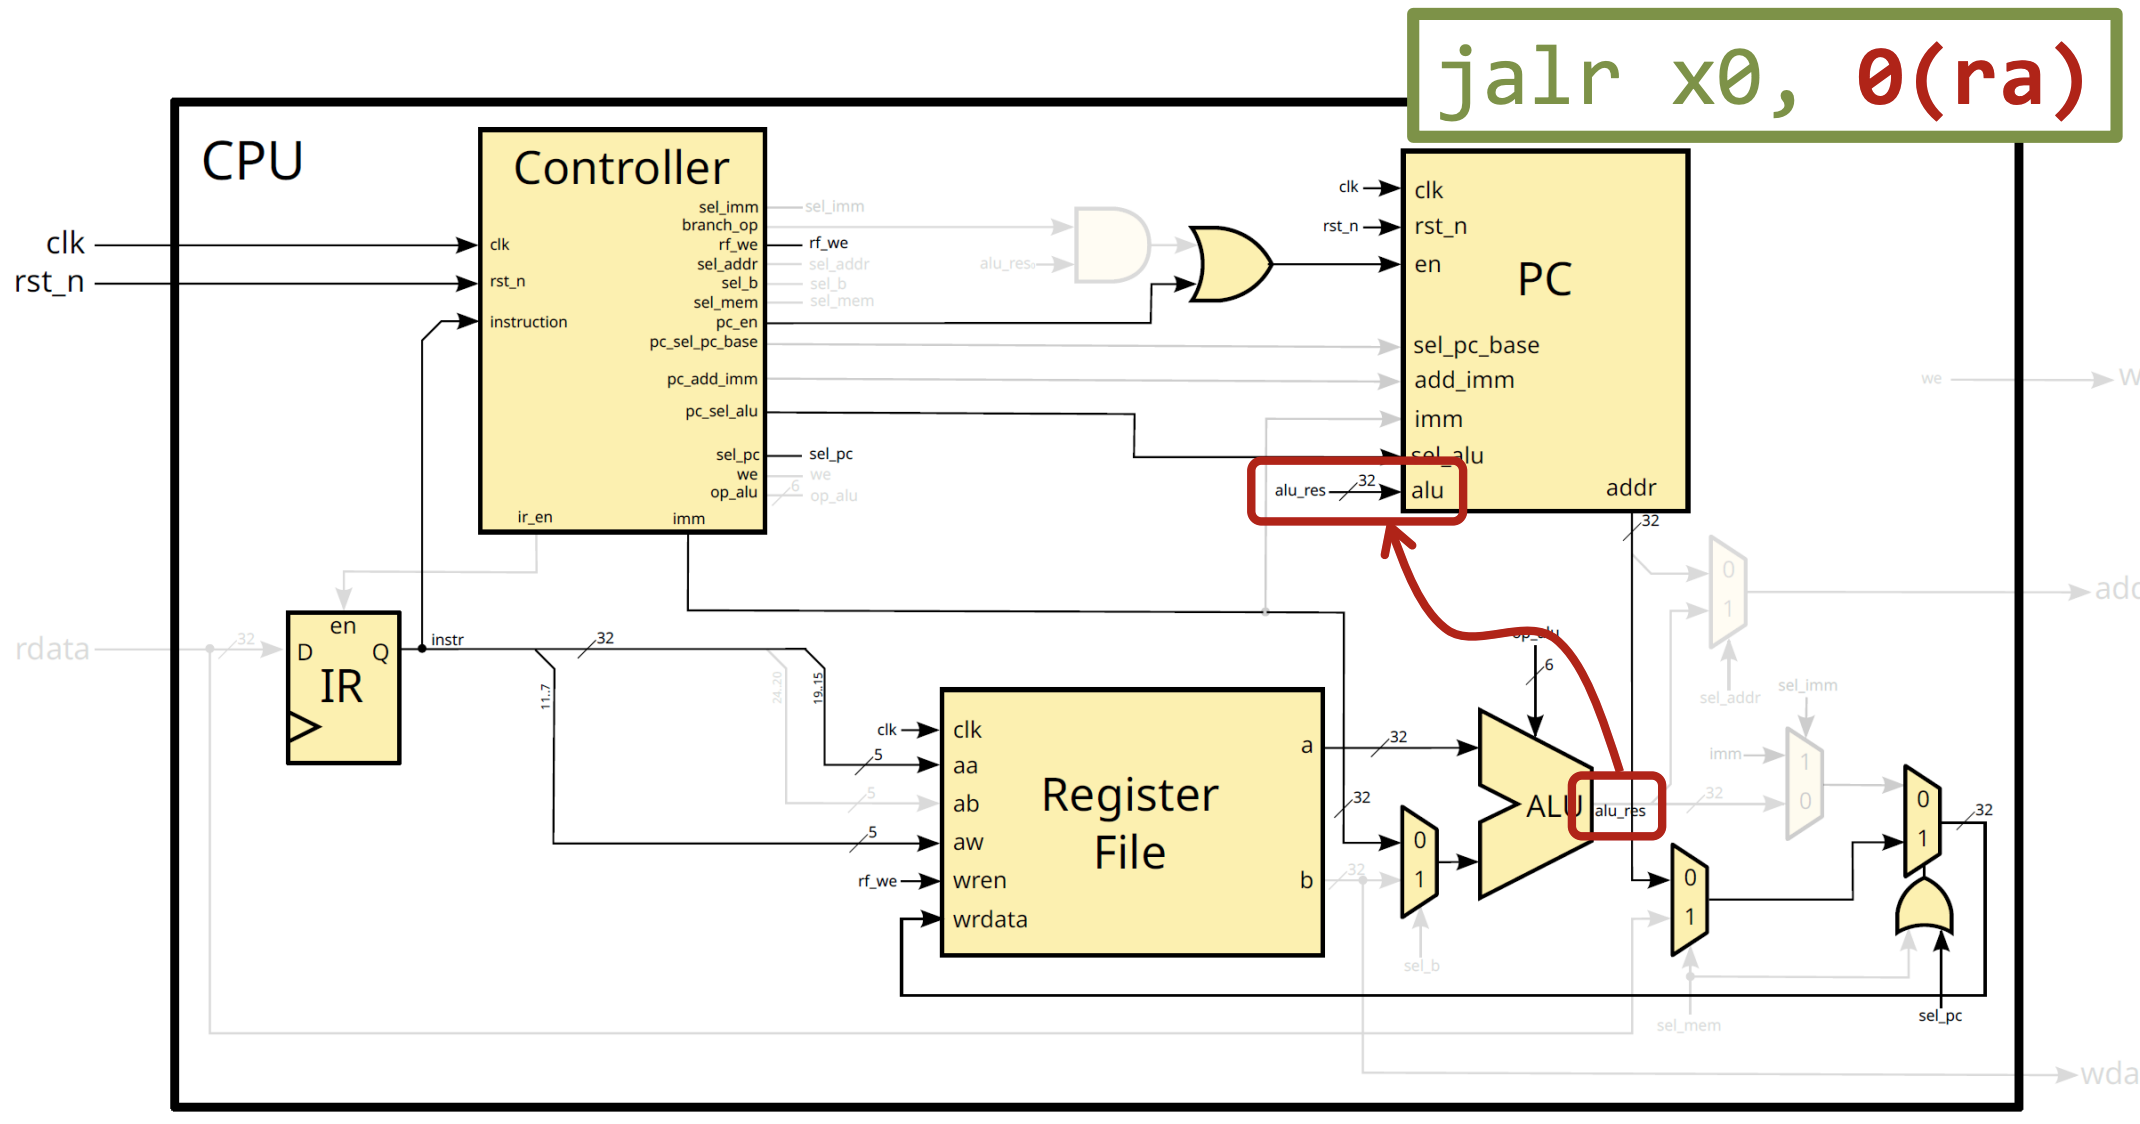
\includegraphics[width=0.75\textwidth]{chapters/chapter2a/images/pend.png}
\end{center}

\subsection{Guidelines for Writing Verilog}
Before beginning to write Verilog code, it is crucial to follow certain guidelines to ensure clarity and correctness in your hardware design. Verilog and VHDL are Hardware Description Languages (HDLs) that require a clear and structured approach. \\
\textit{Anything that's complicated is a Module, anything that is trivial, we need to know if it's sequential or combinational.}
\begin{itemize}
    \item \textbf{Clarity and Preparation:} 
    \begin{itemize}
        \item Ensure that you have drawn a diagram, as demonstrated in previous examples.
        \item Clearly distinguish between \textbf{combinational} and \textbf{sequential} blocks in your design.
    \end{itemize}

    \item \textbf{Decomposition of Complex Sequential Blocks:}
    \begin{itemize}
        \item Break down complex sequential blocks into simpler, well-defined elements. For instance, sequential blocks should primarily consist of simple registers (e.g., Instruction Register - IR).
        \item Continue refining your hierarchical diagrams until all sequential blocks become trivial to implement.
    \end{itemize}

    \item \textbf{Adopt a Hierarchical Approach:}
    \begin{itemize}
        \item Use a hierarchical approach, similar to programming practices, and employ your diagrams to guide the creation of modules, such as the Program Counter (PC).
    \end{itemize}
\end{itemize}

\textit{For example, for our processor, identifying that a register file is sequential while a PC is combinational is crucial before starting to write Verilog.}

\subsection{Detailing Complex Combinational Modules (ALU)}
When designing complex combinational modules, it is essential to clearly define and break down each component to ensure accurate and efficient implementation. The following steps outline the process of detailing these modules:
\begin{center}
    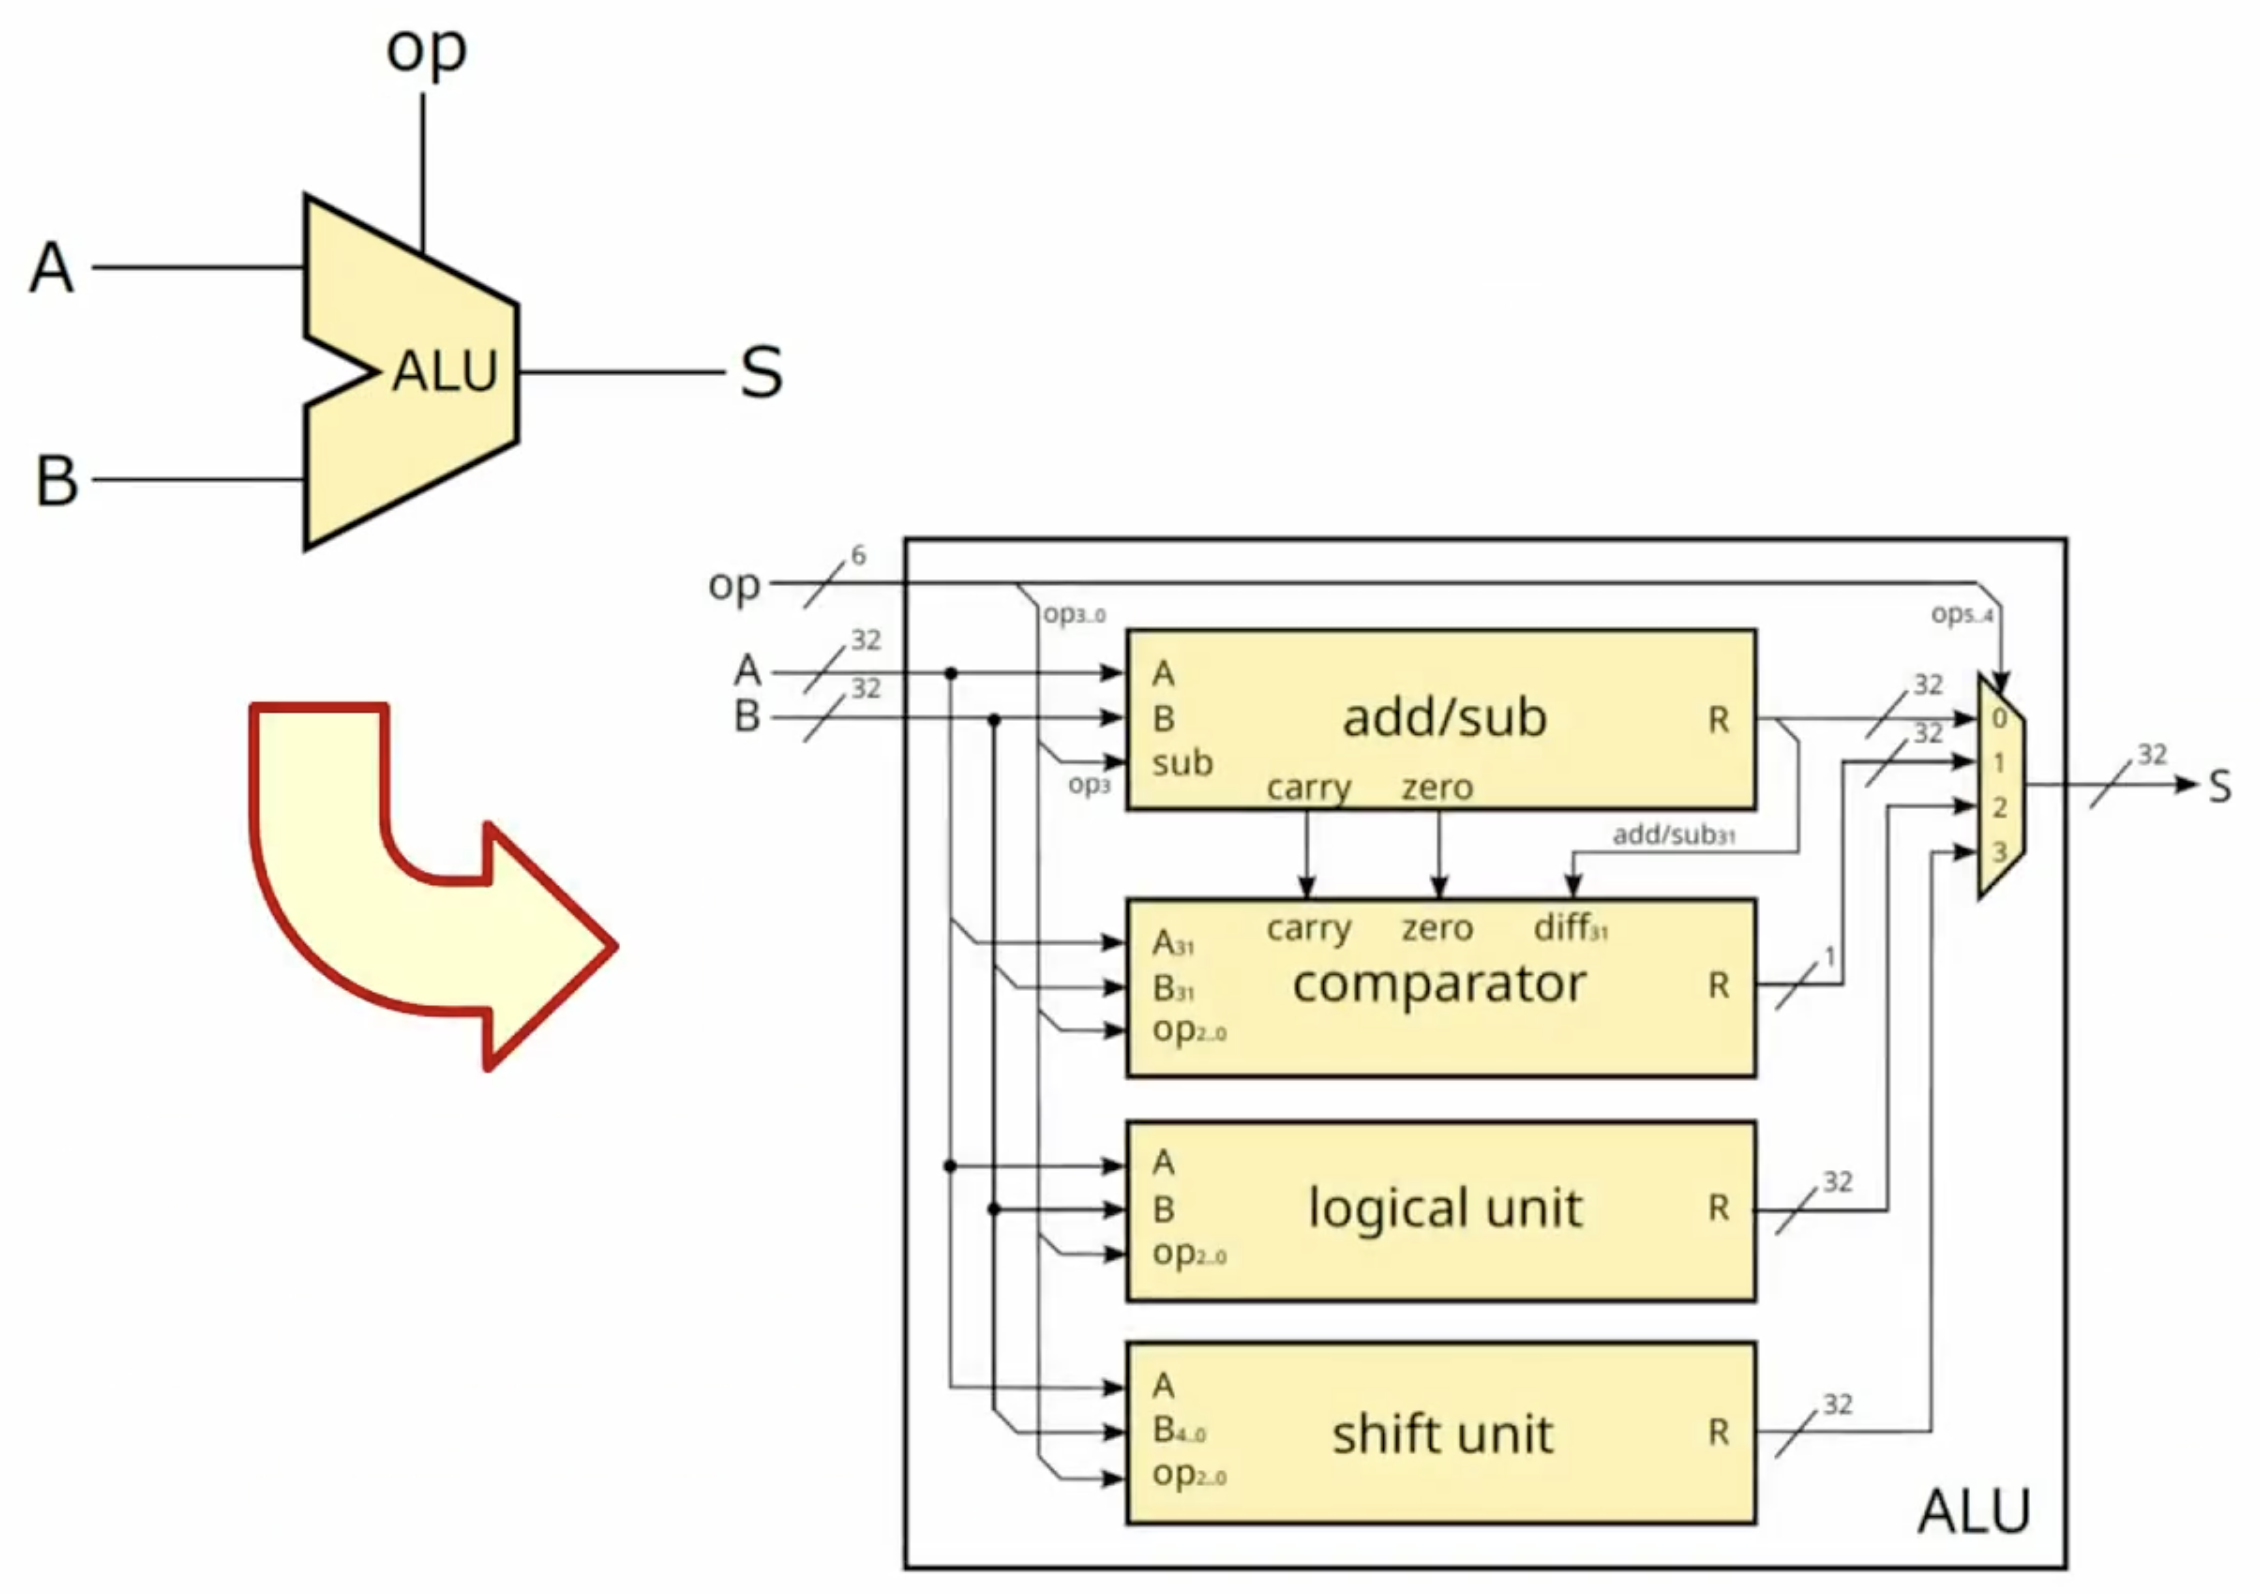
\includegraphics[width=0.45\textwidth]{chapters/chapter2a/images/ALU.png}
\end{center}
\begin{itemize}
    \item \textbf{ALU (Arithmetic Logic Unit) Overview:}
    \begin{itemize}
        \item The ALU receives inputs \( A \), \( B \), and an operation code (\textit{op}), and produces an output \( S \).
        \item It contains multiple submodules, such as add/subtract, comparator, logical unit, and shift unit.
    \end{itemize}

    \item \textbf{Add/Subtract Unit:}
    \begin{itemize}
        \item The add/subtract unit performs addition and subtraction operations based on the control signal \textit{sub}. 
        \item It includes circuitry to handle carry and zero detection, essential for arithmetic operations.
    \end{itemize}

    \item \textbf{Hierarchical Design:}
    \begin{itemize}
        \item The ALU is composed hierarchically, where each submodule (e.g., add/subtract, comparator) performs specific functions and connects to the overall ALU structure.
        \item Such a design allows for easier debugging, maintenance, and understanding of each module’s role within the ALU.
    \end{itemize}
\end{itemize}

\subsection{Verilog - Sticking to Basic Paterns}
When writing Verilog, it is essential to adhere to basic patterns for describing combinational and sequential logic. This section provides guidelines on structuring Verilog code efficiently.

\begin{center}
    \begin{minipage}{0.45\textwidth}
        \textbf{Combinational Logic} \vspace{0.5em} \\
        Combinational logic blocks should be described using the \texttt{always @(*)} construct. This approach ensures that outputs are updated whenever the inputs change.
        \begin{verilog}
always @(*) begin
    if (a) 
        y = \~b;
    else 
        y = b;
end
        \end{verilog}

        Complex combinational blocks, such as the next state in a finite state machine (FSM), can also be described using this pattern.
    \end{minipage}
    \hfill
    \vline
    \hfill
    \begin{minipage}{0.45\textwidth}
\textbf{Sequential Logic} \vspace{0.5em} \\
Sequential logic blocks should be described using the \texttt{always @(posedge clk)} construct. This pattern is suitable for describing registers and counters.

\begin{verilog}
always @(posedge clk) begin
    if (reset == 1) 
        q <= 0;
    else if ((enable1 == 1) && (enable2 == 1)) 
        q <= d;
end
        \end{verilog}

        Use \texttt{posedge clk} to trigger updates on the rising clock edge.
    \end{minipage}
\end{center}

For detailed guidelines, refer to the Verilog guidelines provided in Moodle.
